\documentclass[twoside]{article}
\usepackage[accepted]{aistats2017}
\usepackage[round]{natbib}
\usepackage{listings}
\usepackage{minted}
\usepackage{color}
\usepackage{algorithm}
\usepackage{algpseudocode}
\usepackage{amsmath}
\usepackage{amssymb}
\usepackage{dsfont}
\usepackage{pgf}
\usepackage{subcaption}
%\graphicspath{{report_data_and_plots/}}
%\definecolor{mygreen}{rgb}{0,0.6,0}
%\definecolor{mygray}{rgb}{0.5,0.5,0.5}
%\definecolor{mymauve}{rgb}{0.58,0,0.82}
%
%\lstset{ %
%	backgroundcolor=\color{white},   % choose the background color; you must add \usepackage{color} or \usepackage{xcolor}; should come as last argument
%	basicstyle=\footnotesize,        % the size of the fonts that are used for the code
%	breakatwhitespace=false,         % sets if automatic breaks should only happen at whitespace
%	breaklines=true,                 % sets automatic line breaking
%	captionpos=b,                    % sets the caption-position to bottom
%	commentstyle=\color{mygreen},    % comment style
%	deletekeywords={...},            % if you want to delete keywords from the given language
%	escapeinside={\%*}{*)},          % if you want to add LaTeX within your code
%	extendedchars=true,              % lets you use non-ASCII characters; for 8-bits encodings only, does not work with UTF-8
%	frame=single,	                   % adds a frame around the code
%	keepspaces=true,                 % keeps spaces in text, useful for keeping indentation of code (possibly needs columns=flexible)
%	keywordstyle=\color{blue},       % keyword style
%	language=Octave,                 % the language of the code
%	morekeywords={*,...},            % if you want to add more keywords to the set
%	numbers=left,                    % where to put the line-numbers; possible values are (none, left, right)
%	numbersep=5pt,                   % how far the line-numbers are from the code
%	numberstyle=\tiny\color{mygray}, % the style that is used for the line-numbers
%	rulecolor=\color{black},         % if not set, the frame-color may be changed on line-breaks within not-black text (e.g. comments (green here))
%	showspaces=false,                % show spaces everywhere adding particular underscores; it overrides 'showstringspaces'
%	showstringspaces=false,          % underline spaces within strings only
%	showtabs=false,                  % show tabs within strings adding particular underscores
%	stepnumber=2,                    % the step between two line-numbers. If it's 1, each line will be numbered
%	stringstyle=\color{mymauve},     % string literal style
%	tabsize=2,	                   % sets default tabsize to 2 spaces
%%	title=\lstname                   % show the filename of files included with \lstinputlisting; also try caption instead of title
%}
 % If your paper is accepted, change the options for the package
% aistats2017 as follows:
%
%\usepackage[accepted]{aistats2017}
%
% This option will print headings for the title of your paper and
% headings for the authors names, plus a copyright note at the end of
% the first column of the first page.

\renewcommand{\bibsection}{}
\begin{document}

% If your paper is accepted and the title of your paper is very long,
% the style will print as headings an error message. Use the following
% command to supply a shorter title of your paper so that it can be
% used as headings.
%
%\runningtitle{I use this title instead because the last one was very long}

% If your paper is accepted and the number of authors is large, the
% style will print as headings an error message. Use the following
% command to supply a shorter version of the authors names so that
% they can be used as headings (for example, use only the surnames)
%
%\runningauthor{Surname 1, Surname 2, Surname 3, ...., Surname n}

\twocolumn[

\aistatstitle{Hamiltonian Monte Carlo Inference for a First Order Probabilistic Programming Language }

%\aistatsauthor{ Bradley Gram-Hansen \And Frank Wood \And  Author 3 }
\aistatsauthor{ Bradley Gram-Hansen \And Frank Wood }
%\aistatsaddress{ Institution 1 \And  Institution 2 \And Institution 3 } ]
\aistatsaddress{ Department of Engineering,  University of Oxford } ]
\begin{abstract}
  The Abstract paragraph should be indented 0.25 inch (1.5 picas) on
  both left and right-hand margins. Use 10~point type, with a vertical
  spacing of 11~points. The {\bf Abstract} heading must be centered,
  bold, and in point size 12. Two line spaces precede the
  Abstract. The Abstract must be limited to one paragraph.
\end{abstract}

\section{Introduction}

%\lstinputlisting[language=Python]{test.py}
%Papers are in 2 columns with the overall line width of 6.75~inches (41~picas). Each column is 3.25~inches wide (19.5~picas).  The space
%between the columns is .25~inches wide (1.5~picas).  The left margin is 1~inch (6~picas).  Use 10~point type with a vertical spacing of
%11~points. Please use US Letter size paper instead of A4.
%
%Paper title is 16~point, caps/lc, bold, centered between 2~horizontal rules.  Top rule is 4~points thick and bottom rule is 1~point thick.
%Allow 1/4~inch space above and below title to rules.

Monte Carlo Markov Chain (MCMC) methods are a set of powerful inference algorithms \citep{berg2008markov} that enable us to evaluate, model and analyze complicated probabilistic models such as those found in machine learning and Bayesian inference \citep{andrieu2003introduction} and in natural systems, such as those found in Biology \citep{sorensen2007likelihood} and Physics \citep{duane1987hybrid}. 
However, as the dimensionality of the problem grows many MCMC methods, such as Metropolis-Hastings \citep{hastings1970monte},  become ineffective at being able to generate samples effectively. This can be overcome in some instances by tuning particular parameters or rephrasing the problem in a different manner, but this cannot always be done. One MCMC this is able to circumvent this problem is Hamiltonian Monte Carlo (HMC) \citep{neal2011mcmc}\citep{duane1987hybrid}, which takes inspiration from the physical world and uses a dynamical model to generate new proposals. This in turn enables us to explore larger spaces more effectively globally, rather than getting trapped in local regions. See section \ref{sec:supmat} for more information on HMC. \\
Choosing the right inference algorithm is critical for probabilistic programming languages \citep{tolpin2015probabilistic} such as Anglican \citep{wood2014new} and others, where we rely upon accurate inference and sampling procedures to evaluate our programs. Although, in practice there is no-one inference or sampling algorithm to rule them all. Thus we rely on a combination of techniques, to deal with both finite parameter and infinite parameter spaces (non-parametric models). To analyze more effectively a subset of the problems that Anglican can, such as finite graphs, FOPPL, a first order probabilistic programming language was constructed so that we could take advantage of fast inference algorithms, such as HMC.\\
In this work we make two contributions, we introduce a FOPPL compiler that transforms a FOPPL output, a finite graph, into python code that takes advantage of the Automatic differentiation package within Pytorch \citep{pytorch} and an HMC that correctly deals with conditional statements and can deal with both finite continuous and discrete parameters us


\section{Hamiltonian Monte Carlo}
In a top level view Hamilton Monte Carlo for Monte Carlo Markov Chain (HMC MCMC) is a two step process. In step one we define a Hamiltonian function in terms of the probability distribution from which we wish to sample from. We introduce a position variable, $q$ (our latent parameters) and momentum variable $p$, where $p$ is an auxiliary variable that typically has a Gaussian distribution.  All $p$'s are assumed independent. 
In step two, the HMC alternates simple updates for the momentum variables with Metropolis updates. This enables us to propose a new state by computing a trajectory according to Hamiltonian dynamics, implemented with the leapfrog method. 

The Hamiltonian of a physical system is defined completely with respect to the position $q$ and $p$ momentum variables, which span the phase space of the system. The Hamiltonian is the Legendre transform of the Lagrangian and gives us the total energy in the system, that is \begin{equation}
\label{eq:hamreduced}
H(\textbf{q}, \textbf{p})  = K(p) + U(q)
\end{equation}
where the Legendre transform is defined as follows: 
\begin{equation}
\label{eq:hamiltonian}
H(\textbf{q},\textbf{p}) = \sum_{i = 1}^{d}\dot{q}_{l}p_{l} - L(\textbf{q}, \textbf{\.{q}}(\textbf{q}, \textbf{p}))
\end{equation}
where $d$ is the system dimensions, and so the full state space with has $2d$ dimensions.  
Thus, for simplicity, if we set $d = 1$ we can derive the Hamiltonian equations as follows:\begin{equation}
\label{eq:hameq1}
\frac{\partial H}{\partial p} = \dot{q} + p\frac{\partial \dot{q}}{\partial p} - \frac{\partial L}{\partial \dot{q}}\frac{\partial \dot{q}}{\partial p} = \dot{q} \end{equation}
and 
\begin{equation}
\label{eq:hameq2}
\frac{\partial H}{\partial q} = p\frac{\partial \dot{q}}{\partial q} - \frac{\partial L}{\partial q} - \frac{\partial L}{\partial \dot{q}}\frac{\partial \dot{q}}{\partial q} = - \frac{\partial L}{\partial q}= -\dot{p}  \end{equation}
and the process is the same for more than one dimension. 
where $K(p)$ represents our kinetic energy and $U(q)$ is the potential energy.

Within the HMC MCMC framework the ''positions", $q$, are the variables of interest and for each position variable we have to create a fictitious ''momentum", $p$. For compactness let $z = (q,p)$. The potential energy $U(q)$ will be the minus of the log of the probabilty density for the distribution of the position variables we wish to sample, plus \textbf{any} constant that is convenient.  The kinetic energy will represents the dynamics of our variables, for which a popular form of $K(p) = \frac{p^{T} M^{-1} p}{2}$, where $M$ is symmetric, positive definite and typically diagonal. This form of $K(p)$ corresponds to a minus the log probability of the zero mean Gaussian distribution with covariance matrix $M$. For this choice we can write the Hamiltonian equations, for any dimension $d$, as follows:
\begin{align}
\label{eq:ham1neal}
\dot{q}_{i} &= \frac{dq_{i}}{dt} = [M^{-1}p]_{i}\\
\label{eq:ham2neal}
\dot{p}_{i} &= \frac{dp_{i}}{dt} = -\frac{\partial U}{\partial q_{i}}
\end{align}

To view the Hamiltonian in terms of probabilities, we use the concept of the canonical distribution from Statistical mechanics to construct our pdf. Thus, the distribution that we wish to sample from can be related to the potential energy via the canonical distribution as:
\begin{equation}
\label{eq:canonical}
P(z) = \frac{1}{Z}\exp\left(\frac{-E(z)}{T}\right)
\end{equation}
As the Hamiltonian is just an energy function we may can insert \ref{eq:hamreduced}\ into our canonical distribution \ref{eq:canonical}\, which gives us the joint density:
\begin{equation}
P(q,p) = \frac{1}{Z}\exp(-U(q))\exp(-K(p)  
\end{equation}
where $T = 1$ is fixed. And so we can now very easily get to our target distribution $p(q)$, which is dependent on our choice of potential $U(q)$, as this expression factorizes in to two independent probability distributions. 
We characterise the posterior distribution for the model parameters using the potential energy function: \begin{equation}
U(q) = -\log[\pi(q)L(q|D)]
\end{equation}
where $\pi(q)$ is the prior distribution, and $L(q|D)$ is the likelihood, not the Lagrangian, of the given data $D$. 

\subsection{The Integrator}

\textbf{Talk about the properties of integrators, why they are important and why we are using the leapfrog integrator.}
The leapfrog method enables us to discretise Hamiltons equations and as it is a valid integrator, it allows us to numerically solve Hamiltons equations \ref{eq:ham1neal} and \ref{eq:ham2neal}. In doing so, we generate new proposals given some initial state 
We start with a state at $t = 0$ and then evaluate at a subsequent time $t + \epsilon , \hdots, t + n\epsilon$, where $\epsilon$ is the step in which we increase and $n$ is the number of time steps. 

\begin{align}
p_{i}(t + \frac{\epsilon}{2}) &= p_{i}(t) - \left(\frac{\epsilon}{2}\right)\frac{\partial U(q(t))}{\partial q_{i}} \\
q_{i}(t + \epsilon) &= q_{i}(t) + \epsilon\frac{\partial K(p(t + \frac{\epsilon}{2}))}{dp_{i}}\\
p_{i}(t + \epsilon) &= p_{i}(t + \frac{\epsilon}{2}) - \left(\frac{\epsilon}{2}\right)\frac{\partial U(q(t+\epsilon))}{\partial q_{i}}
\end{align}
\footnote{For the usual choice of kinetic energy, we have $\frac{\partial K(p + \frac{\epsilon}{2})}{dp_{i}} = \frac{p_{i}(t + \frac{\epsilon}{2})}{m_{i}}$}

For the leapfrog method the local error, error after one step, is of $\mathcal{O}(\epsilon^{2})$ and a global error, error after simulating for some fixed time interval s, which requires $\frac{s}{\epsilon}$ is $\mathcal{O}(\epsilon^{3})$
Neals implementation of the HMC can only be used to sample from continuous distributions on $\mathbb{R}^{d}$ for which a density function can be evaluated.\\
We must be able to compute the partial derivative of the log of the density function, the joint. 
HMC samples from the canonical distribution for $q$ and $p$. $q$ has the distribution of interest as specified by the potential $U(q)$. 
The distribution of the $p$'s can be chosen by us and are independent of the $q$'s. 
The $p$ components are specified to be independent, with component $p_{i}$ having variance $m_{i}$.
The kinetic energy $K(p) = \sum_{i =1}^{d}\frac{p_{i}^{2}}{2m_{i}}(q(t + \epsilon))
$
\subsubsection{Properties of the Integrator}
Reversibility

\subsubsection{The Algorithm}

\begin{enumerate}
	\item Step 1: Changes only the momentum
	\item Step 2: May change both position and momentum
\end{enumerate}
Both steps leave the canonical distribution of (q,p) invariant, hence the distribution remains invariant.

In \textbf{Step 1} we first draw the $p_{i}$ randomly from their Gaussian distribution independently of the current values of the position values. 
In \textbf{Step 2} a Metropolis update is performed, using the Hamiltonian dynamics to propose a new state. Starting with the current state $(q,p)$, Hamiltonian dynamics is simulated for $L$ steps using the leapfrog method, with a stepsize of $\epsilon$. $L$ and $\epsilon$ are parameters of the mnodel that need to be tuned.\\
The momentum vairables at the end of this $L$-step trajectory are then negated, giving s proposed state $(q^{*}. p^{*})$. This proposed state is accepted as the next state in the Markov Chain with probability: \begin{multline}
\min[1, \exp(-H(q^{*}, p^{*}) + H(p,q)] =\\
\min[1, \exp(-U(q^{*}) + U(q) - K(p^{*}) + K(p))]
\end{multline} 
\begin{algorithm}
	\label{alg:simpHMC}
	\caption{\textbf{Continuous Hamiltonian Monte Carlo MCMC}}
	\begin{algorithmic}[1]
		\Procedure{HMC}{$x_{0}$, $\epsilon$, $L$,$U$, $M$}
		\For{$m = 1 \text{ to } M$}
		\State $ p^{0} \sim \mathcal{N}(0,\mathds{1})$
		\State $ x^{m} \gets x^{m-1}$
		\State $x^{'} \gets x^{m-1}$
		\State $ p^{'} \gets p^{0}$
		\For {$i = 1 \text{ to } L$}
		\State $x^{'}$ , $p \gets$ Leapfrog($x^{'}, p^{'}, \epsilon$)
		\EndFor
		\State $\alpha = \min\left\{1, \frac{\exp \left\{-U(x^{'}) - K(p^{'})\right\}}{\exp \left\{U(x^{m-1}) - K(p^{0})\right\}}\right\}$
		\State $u \sim Uniform(0,1)$
		\If{ $u < \alpha $}
		\State \Return $ x^{m} \gets x^{'}$, $p^{m} \gets -p $  \Comment{Accept}
		\Else
		\State \Return $x^{m}  \gets x^{m-1}$ , $p^{m} \gets p^{0}$ \Comment{Reject}
		\EndIf
		\EndFor
		\State {Leapfrog($x$, $p$, $\epsilon$)} 
		\State $p^{'} \gets p - \frac{\epsilon}{2}\nabla_{x} U(x)$ \Comment{Half step for momentum}
		\State $x^{'} \gets x + \epsilon \nabla_{p} K(p^{'})$ \Comment{Full step for position} 
		\State $p^{'} \gets p - \frac{\epsilon}{2}\nabla_{x}U(x^{'})$ \Comment{Half step for momentum}
		\State \Return $x^{'}$ , $p^{'}$
	\end{algorithmic} 
\end{algorithm}
If the proposed state is rejected, then the next state is the same as the current state and is counted again when calculating the expected value of some function. 
The negation of the momentum variables at the end of the trajectory makes the Metropolis proposal symmetrical, as needed for the acceptance probability above to be valid. This negation need not be done in practice, since $K(p) = K(-p)$, and the momentum will be replaced before it is used again, in the first step of the next iteration.
Where $U = -\log(\pi(x))$,  $M$ is the number of samples we wish to take , $(x^{'}, p^{'})$ is the generated proposal and we propose setting $x^{m} = x^{'}$ and $p^{m} = -p^{'}$ and then accept or reject this proposal according to the Metropolis update step. 
A function that implements a single iteration of the HMC algorithm is given in algorithm 2. There are three additional functions within this iteration: $U$, which returns the potential energy given a value for $q$,  $\nabla U$, which returns the vector of partial derivatives of $U$ given $q$ and $\nabla K$, which returns the vector of partial derivatives of $K$ given $p$. Other arguments are the stepsize, $\epsilon$, for leapfrog steps, the number of leapfrog steps in the trajectory, $L$, and the current position, $q_{current}$, that the trajectory starts from. Momentum variables are sampled within this function, and discarded at the end, with only the next position being returned. 

\section{Example Programs and Compiled Output}

\subsection{Programs}

We now present a few simple FOPPL programs and discuss both their statistical and syntactic structures. 

\subsection{Conjugate Gaussian}
The conjugate Gaussian, is a model in which we can analytically calculate the true posterior $p(x | y) \propto p(x,y) $, as the product of two Gaussians is also a Gaussian. For our particular model we \mintinline{clojure}{sample} $x \sim \mathcal{N}(0, 1)$ and we \mintinline{clojure}{observe} $y = 7$, with likelihood $p(y|x) = \mathcal{N}(y | x, 1)$.  In FOPPL we have the following output:
\inputminted{clojure}{code/conjugategauss.clj}

Thus, the joint $ p(x,y) \propto p(x|y) = p(x)p(y| x) = \mathcal{N}(\bar{\mu}, \bar{\sigma}^{2})$, where $\bar{\mu} = \left(\frac{\mu_{0}\sigma^{2} + \sigma^{2}_{0}\sum_{i=1}^{n}y_{i}}{\sigma^{2}\sigma^{2}_{0}}\right) \bar{\sigma}^{2}$ and $\bar{\sigma}^{2} = \left(\frac{1}{\sigma^{2}_{0}} + \frac{n}{\sigma^{2}}\right)^{-1} $. Where in this model $n$ is the total number of observed datum $y$, $\mu_{0} = 0 $ and $\sigma_{0}^{2} = 1$ are the prior mean and variance and $\sigma^{2} = 1.0 $ is the likelihood variance. Thus the true mean that our model should infer is $\bar{\mu} = 5$. 
\subsection{Conditional If}
The \mintinline{clojure}{if} statement is typically challenging to implement for gradient based methods, due to the branching effects that occur at the condition. For trace based samplers, such as importance sampling, this is not a problem as multiple traces are recorded for each path taken. However, in higher dimensions these types of samplers are heavily impaired. 
\inputminted{clojure}{code/conditionalif.clj}
I
\subsection{Linear Regression}
\inputminted{clojure}{code/linearregression.clj}


\subsubsection{Models and Results}

Here we introduce a section of simple models and the results of inference via our custom built HMC sampler on those programs. For a sample output of the compiler for the linear regression program, please see section \ref{sec:supmat}. 
\paragraph{Fourth Level Heading}
\begin{figure*}[ht]
	\centering
	\subcaptionbox{Fig1}[.3\linewidth][c]{%
		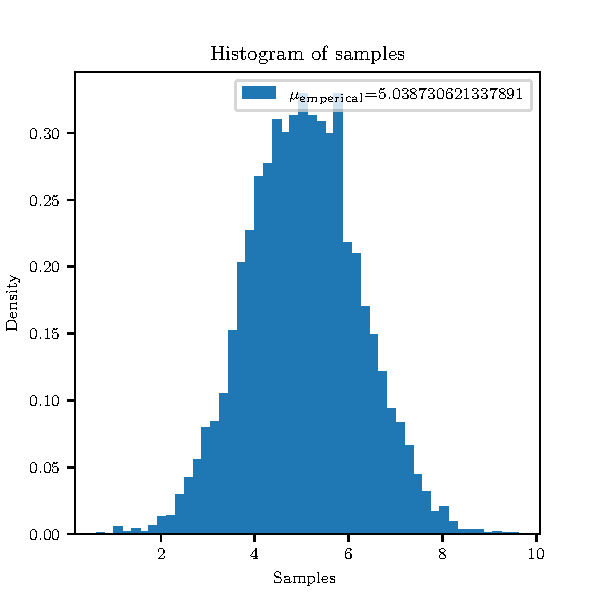
\includegraphics[width=.2\linewidth]{conjgauss/figures/histogram.pdf}}\quad
	\subcaptionbox{Fig2}[.3\linewidth][c]{%
		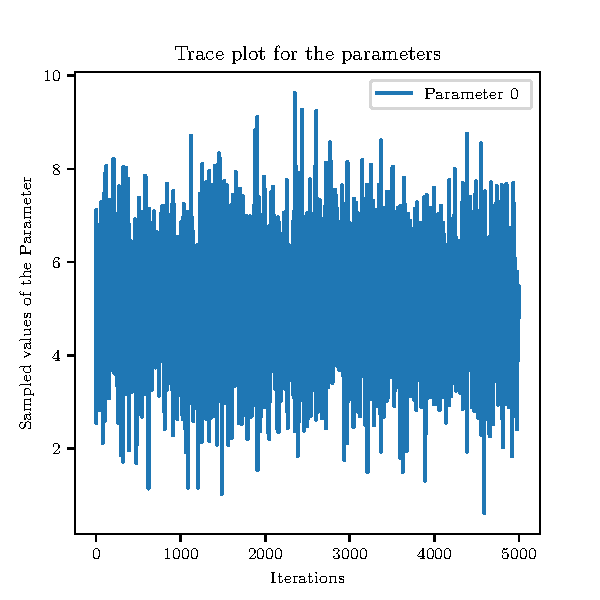
\includegraphics[width=.2\linewidth]{conjgauss/figures/trace.pdf}}\quad
	\subcaptionbox{Fig3}[.3\linewidth][c]{%
		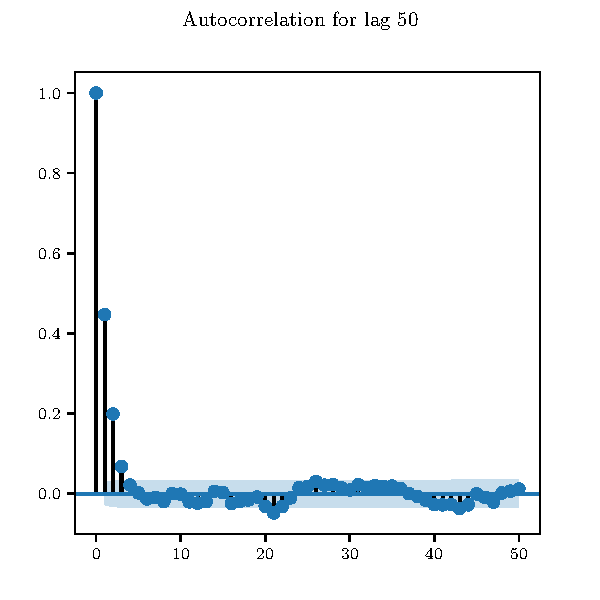
\includegraphics[width=.2\linewidth]{conjgauss/figures/Autocorrelationplot.pdf}}
	
	\bigskip
	
	\subcaptionbox{Fig4}[.3\linewidth][c]{%
		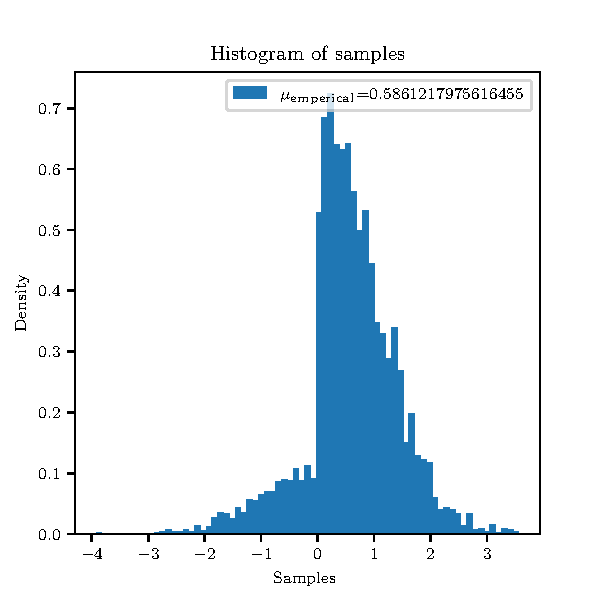
\includegraphics[width=.2\linewidth]{conditionalif/figures/histogram.pdf}}\quad
	\subcaptionbox{Fig5}[.3\linewidth][c]{%
		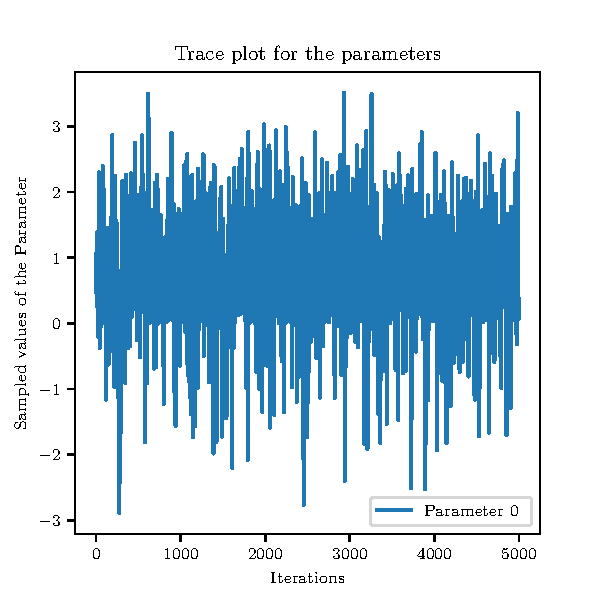
\includegraphics[width=.2\linewidth]{conditionalif/figures/trace.pdf}}\quad
	\subcaptionbox{Fig6}[.3\linewidth][c]{%
		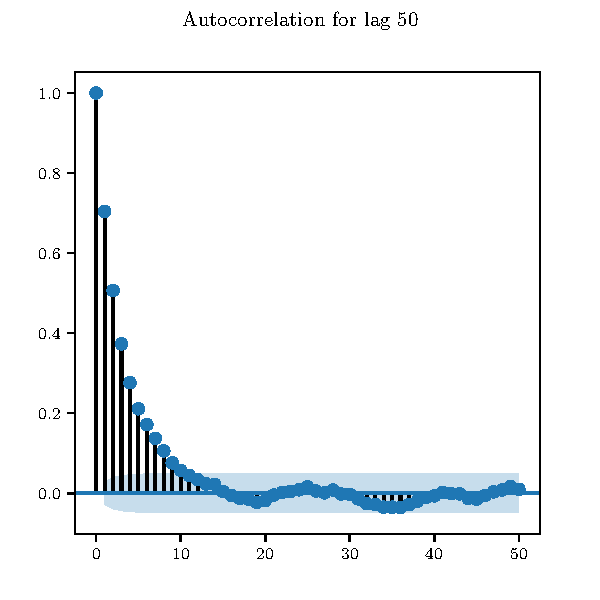
\includegraphics[width=.2\linewidth]{conditionalif/figures/Autocorrelationplot.pdf}}
	
	\bigskip
	
    \subcaptionbox{Fig1}[.3\linewidth][c]{%
		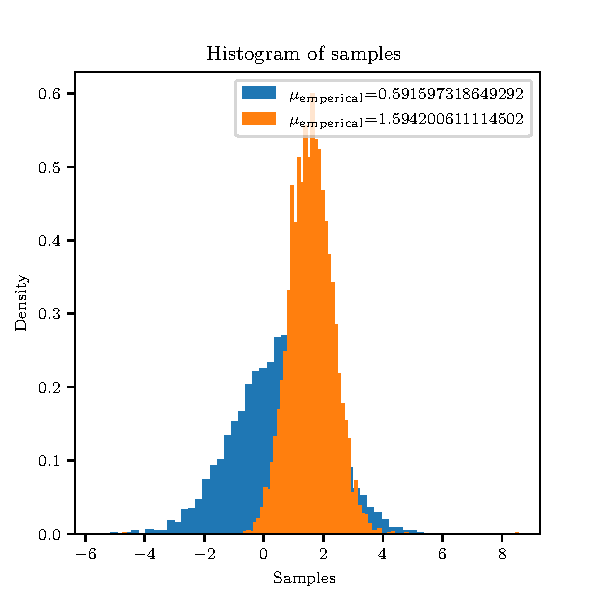
\includegraphics[width=.2\linewidth]{linearreg/figures/histogram.pdf}}\quad
	\subcaptionbox{Fig2}[.3\linewidth][c]{%
		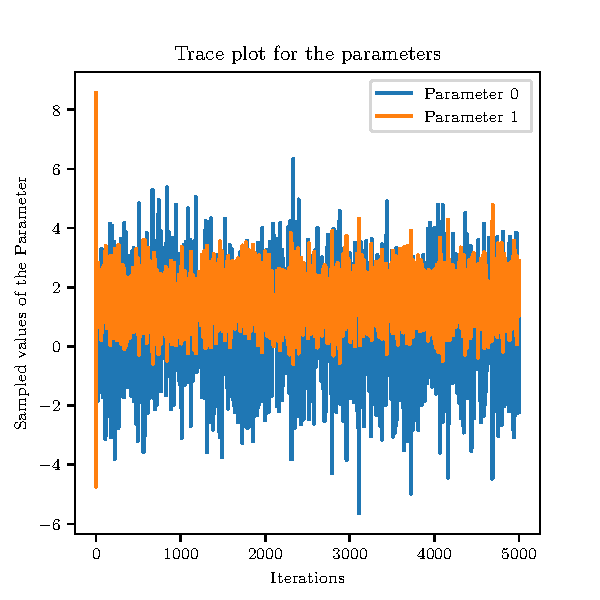
\includegraphics[width=.2\linewidth]{linearreg/figures/trace.pdf}}\quad
	\subcaptionbox{Fig3}[.3\linewidth][c]{%
		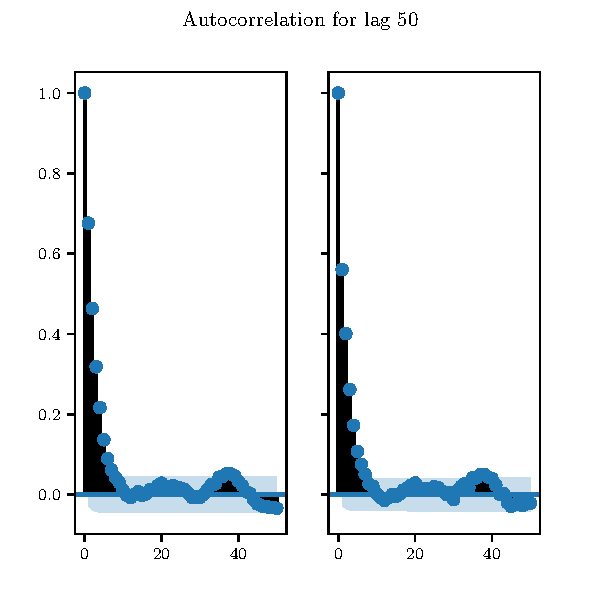
\includegraphics[width=.2\linewidth]{linearreg/figures/Autocorrelationplot.pdf}}
	\caption{All plots}
\end{figure*}
%\begin{figure}[ht]
%	\centering
%	\begin{minipage}{0.33\textwidth}
%		\centering
%		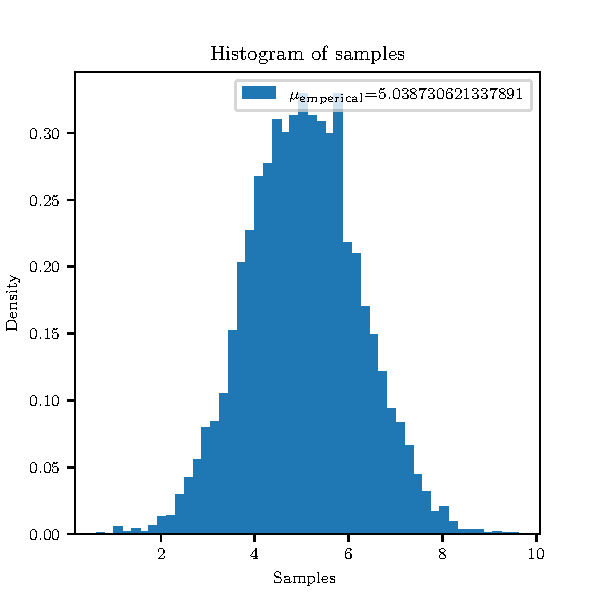
\includegraphics[width=0.9\textwidth]{conjgauss/figures/histogram.pdf} % first figure itself
%	\end{minipage}\hfill
%	\begin{minipage}{0.33\textwidth}
%		\centering
%		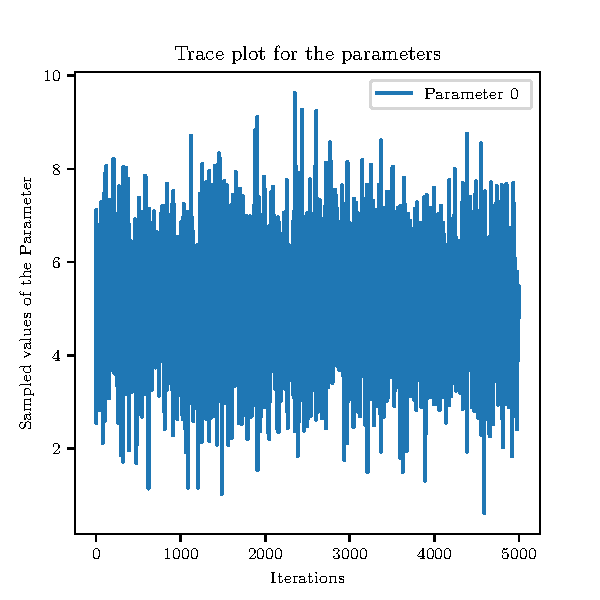
\includegraphics[width=0.9\textwidth]{conjgauss/figures/trace.pdf} % second figure itself
%	\end{minipage}
%	\begin{minipage}{0.33\textwidth}
%	\centering
%	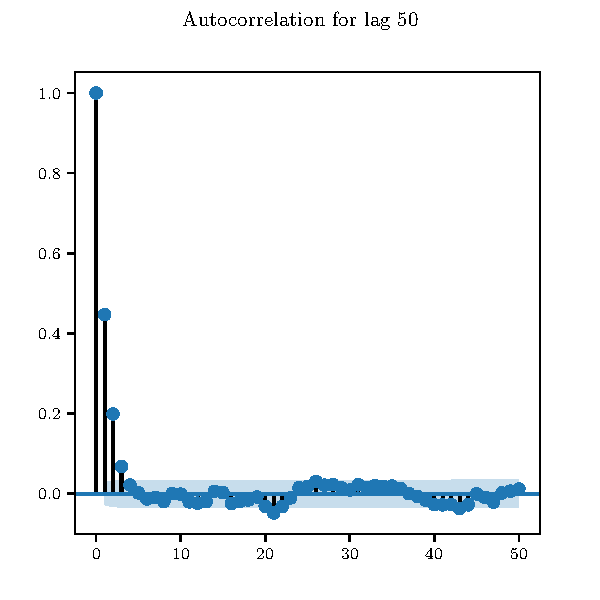
\includegraphics[width=0.9\textwidth]{conjgauss/figures/Autocorrelationplot.pdf} % second figure itself
%\end{minipage}
%\end{figure}
%\begin{figure}[ht]
%	\centering
%	\begin{minipage}{0.33\textwidth}
%		\centering
%		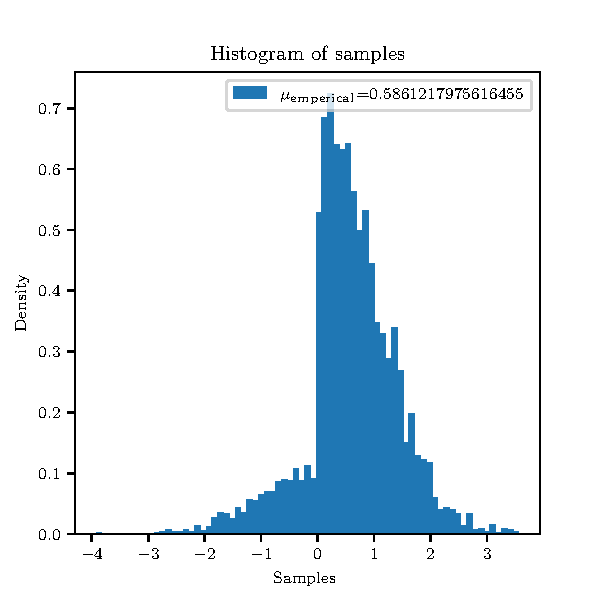
\includegraphics[width=0.9\textwidth]{conditionalif/figures/histogram.pdf} % first figure itself
%	\end{minipage}\hfill
%	\begin{minipage}{0.33\textwidth}
%		\centering
%		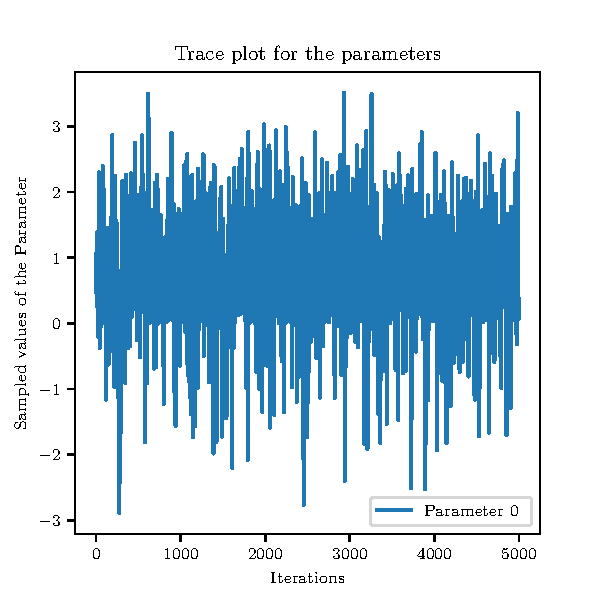
\includegraphics[width=0.9\textwidth]{conditionalif/figures/trace.pdf} % second figure itself
%	\end{minipage}
%	\begin{minipage}{0.33\textwidth}
%	\centering
%	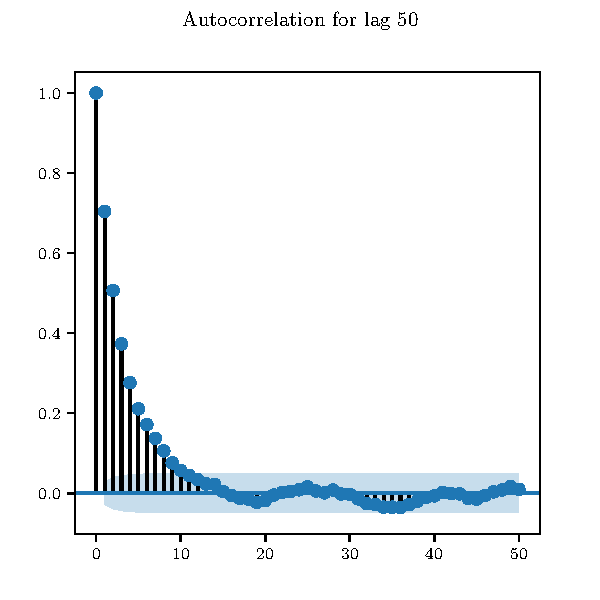
\includegraphics[width=0.9\textwidth]{conditionalif/figures/Autocorrelationplot.pdf} % second figure itself
%\end{minipage}
%\end{figure}
%\begin{figure}[ht]
%	\centering
%	\begin{minipage}{0.33\textwidth}
%		\centering
%		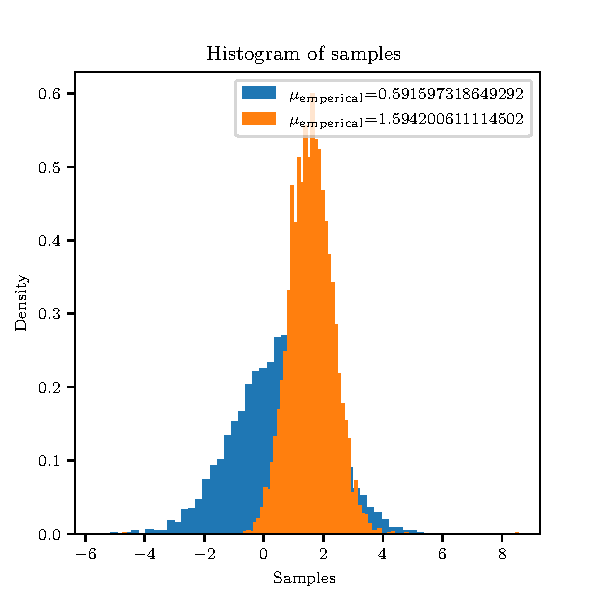
\includegraphics[width=0.9\textwidth]{linearreg/figures/histogram.pdf} % first figure itself
%	\end{minipage}\hfill
%	\begin{minipage}{0.33\textwidth}
%		\centering
%		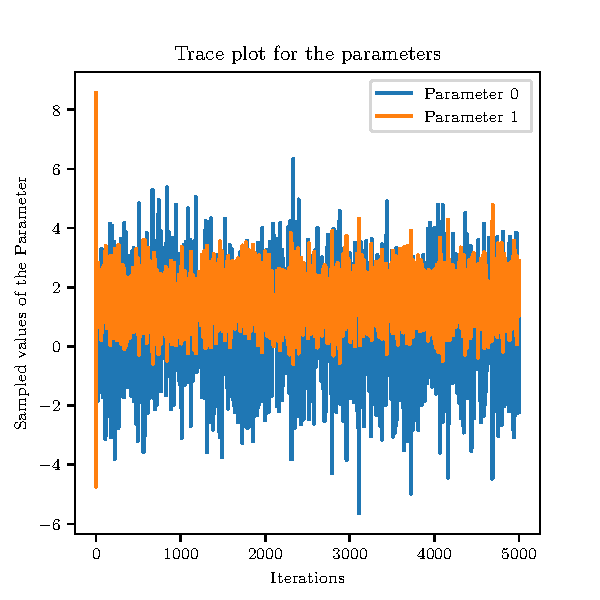
\includegraphics[width=0.9\textwidth]{linearreg/figures/trace.pdf} % second figure itself
%	\end{minipage}
%	\begin{minipage}{0.33\textwidth}
%	\centering
%	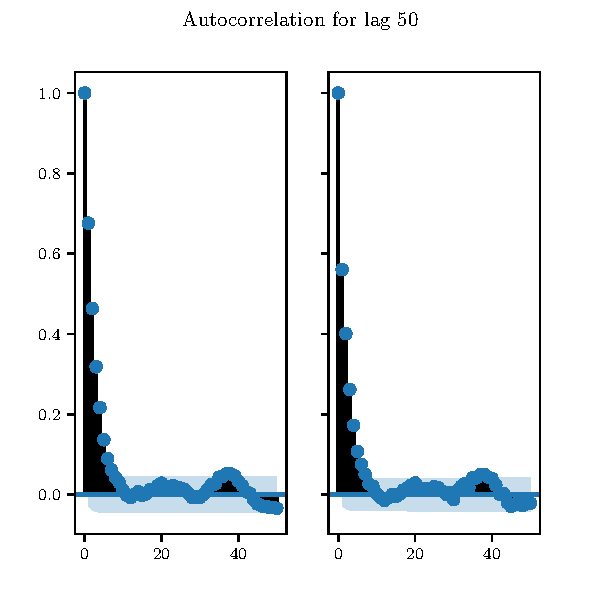
\includegraphics[width=0.9\textwidth]{linearreg/figures/Autocorrelationplot.pdf} % second figure itself
%\end{minipage}
%\end{figure}
%%\end{figure}
%\begin{figure}[ht]
%	\begin{center}
%		%% Creator: Matplotlib, PGF backend
%%
%% To include the figure in your LaTeX document, write
%%   \input{<filename>.pgf}
%%
%% Make sure the required packages are loaded in your preamble
%%   \usepackage{pgf}
%%
%% Figures using additional raster images can only be included by \input if
%% they are in the same directory as the main LaTeX file. For loading figures
%% from other directories you can use the `import` package
%%   \usepackage{import}
%% and then include the figures with
%%   \import{<path to file>}{<filename>.pgf}
%%
%% Matplotlib used the following preamble
%%   \usepackage[utf8x]{inputenc}
%%   \usepackage[T1]{fontenc}
%%
\begingroup%
\makeatletter%
\begin{pgfpicture}%
\pgfpathrectangle{\pgfpointorigin}{\pgfqpoint{4.000000in}{4.000000in}}%
\pgfusepath{use as bounding box, clip}%
\begin{pgfscope}%
\pgfsetbuttcap%
\pgfsetmiterjoin%
\definecolor{currentfill}{rgb}{1.000000,1.000000,1.000000}%
\pgfsetfillcolor{currentfill}%
\pgfsetlinewidth{0.000000pt}%
\definecolor{currentstroke}{rgb}{1.000000,1.000000,1.000000}%
\pgfsetstrokecolor{currentstroke}%
\pgfsetdash{}{0pt}%
\pgfpathmoveto{\pgfqpoint{0.000000in}{0.000000in}}%
\pgfpathlineto{\pgfqpoint{4.000000in}{0.000000in}}%
\pgfpathlineto{\pgfqpoint{4.000000in}{4.000000in}}%
\pgfpathlineto{\pgfqpoint{0.000000in}{4.000000in}}%
\pgfpathclose%
\pgfusepath{fill}%
\end{pgfscope}%
\begin{pgfscope}%
\pgfsetbuttcap%
\pgfsetmiterjoin%
\definecolor{currentfill}{rgb}{1.000000,1.000000,1.000000}%
\pgfsetfillcolor{currentfill}%
\pgfsetlinewidth{0.000000pt}%
\definecolor{currentstroke}{rgb}{0.000000,0.000000,0.000000}%
\pgfsetstrokecolor{currentstroke}%
\pgfsetstrokeopacity{0.000000}%
\pgfsetdash{}{0pt}%
\pgfpathmoveto{\pgfqpoint{0.500000in}{0.440000in}}%
\pgfpathlineto{\pgfqpoint{3.600000in}{0.440000in}}%
\pgfpathlineto{\pgfqpoint{3.600000in}{3.520000in}}%
\pgfpathlineto{\pgfqpoint{0.500000in}{3.520000in}}%
\pgfpathclose%
\pgfusepath{fill}%
\end{pgfscope}%
\begin{pgfscope}%
\pgfpathrectangle{\pgfqpoint{0.500000in}{0.440000in}}{\pgfqpoint{3.100000in}{3.080000in}} %
\pgfusepath{clip}%
\pgfsetbuttcap%
\pgfsetmiterjoin%
\definecolor{currentfill}{rgb}{0.121569,0.466667,0.705882}%
\pgfsetfillcolor{currentfill}%
\pgfsetlinewidth{0.000000pt}%
\definecolor{currentstroke}{rgb}{0.000000,0.000000,0.000000}%
\pgfsetstrokecolor{currentstroke}%
\pgfsetstrokeopacity{0.000000}%
\pgfsetdash{}{0pt}%
\pgfpathmoveto{\pgfqpoint{0.640909in}{0.440000in}}%
\pgfpathlineto{\pgfqpoint{0.687109in}{0.440000in}}%
\pgfpathlineto{\pgfqpoint{0.687109in}{0.448357in}}%
\pgfpathlineto{\pgfqpoint{0.640909in}{0.448357in}}%
\pgfpathclose%
\pgfusepath{fill}%
\end{pgfscope}%
\begin{pgfscope}%
\pgfpathrectangle{\pgfqpoint{0.500000in}{0.440000in}}{\pgfqpoint{3.100000in}{3.080000in}} %
\pgfusepath{clip}%
\pgfsetbuttcap%
\pgfsetmiterjoin%
\definecolor{currentfill}{rgb}{0.121569,0.466667,0.705882}%
\pgfsetfillcolor{currentfill}%
\pgfsetlinewidth{0.000000pt}%
\definecolor{currentstroke}{rgb}{0.000000,0.000000,0.000000}%
\pgfsetstrokecolor{currentstroke}%
\pgfsetstrokeopacity{0.000000}%
\pgfsetdash{}{0pt}%
\pgfpathmoveto{\pgfqpoint{0.687109in}{0.440000in}}%
\pgfpathlineto{\pgfqpoint{0.733308in}{0.440000in}}%
\pgfpathlineto{\pgfqpoint{0.733308in}{0.448357in}}%
\pgfpathlineto{\pgfqpoint{0.687109in}{0.448357in}}%
\pgfpathclose%
\pgfusepath{fill}%
\end{pgfscope}%
\begin{pgfscope}%
\pgfpathrectangle{\pgfqpoint{0.500000in}{0.440000in}}{\pgfqpoint{3.100000in}{3.080000in}} %
\pgfusepath{clip}%
\pgfsetbuttcap%
\pgfsetmiterjoin%
\definecolor{currentfill}{rgb}{0.121569,0.466667,0.705882}%
\pgfsetfillcolor{currentfill}%
\pgfsetlinewidth{0.000000pt}%
\definecolor{currentstroke}{rgb}{0.000000,0.000000,0.000000}%
\pgfsetstrokecolor{currentstroke}%
\pgfsetstrokeopacity{0.000000}%
\pgfsetdash{}{0pt}%
\pgfpathmoveto{\pgfqpoint{0.733308in}{0.440000in}}%
\pgfpathlineto{\pgfqpoint{0.779508in}{0.440000in}}%
\pgfpathlineto{\pgfqpoint{0.779508in}{0.448357in}}%
\pgfpathlineto{\pgfqpoint{0.733308in}{0.448357in}}%
\pgfpathclose%
\pgfusepath{fill}%
\end{pgfscope}%
\begin{pgfscope}%
\pgfpathrectangle{\pgfqpoint{0.500000in}{0.440000in}}{\pgfqpoint{3.100000in}{3.080000in}} %
\pgfusepath{clip}%
\pgfsetbuttcap%
\pgfsetmiterjoin%
\definecolor{currentfill}{rgb}{0.121569,0.466667,0.705882}%
\pgfsetfillcolor{currentfill}%
\pgfsetlinewidth{0.000000pt}%
\definecolor{currentstroke}{rgb}{0.000000,0.000000,0.000000}%
\pgfsetstrokecolor{currentstroke}%
\pgfsetstrokeopacity{0.000000}%
\pgfsetdash{}{0pt}%
\pgfpathmoveto{\pgfqpoint{0.779508in}{0.440000in}}%
\pgfpathlineto{\pgfqpoint{0.825708in}{0.440000in}}%
\pgfpathlineto{\pgfqpoint{0.825708in}{0.456714in}}%
\pgfpathlineto{\pgfqpoint{0.779508in}{0.456714in}}%
\pgfpathclose%
\pgfusepath{fill}%
\end{pgfscope}%
\begin{pgfscope}%
\pgfpathrectangle{\pgfqpoint{0.500000in}{0.440000in}}{\pgfqpoint{3.100000in}{3.080000in}} %
\pgfusepath{clip}%
\pgfsetbuttcap%
\pgfsetmiterjoin%
\definecolor{currentfill}{rgb}{0.121569,0.466667,0.705882}%
\pgfsetfillcolor{currentfill}%
\pgfsetlinewidth{0.000000pt}%
\definecolor{currentstroke}{rgb}{0.000000,0.000000,0.000000}%
\pgfsetstrokecolor{currentstroke}%
\pgfsetstrokeopacity{0.000000}%
\pgfsetdash{}{0pt}%
\pgfpathmoveto{\pgfqpoint{0.825708in}{0.440000in}}%
\pgfpathlineto{\pgfqpoint{0.871908in}{0.440000in}}%
\pgfpathlineto{\pgfqpoint{0.871908in}{0.465071in}}%
\pgfpathlineto{\pgfqpoint{0.825708in}{0.465071in}}%
\pgfpathclose%
\pgfusepath{fill}%
\end{pgfscope}%
\begin{pgfscope}%
\pgfpathrectangle{\pgfqpoint{0.500000in}{0.440000in}}{\pgfqpoint{3.100000in}{3.080000in}} %
\pgfusepath{clip}%
\pgfsetbuttcap%
\pgfsetmiterjoin%
\definecolor{currentfill}{rgb}{0.121569,0.466667,0.705882}%
\pgfsetfillcolor{currentfill}%
\pgfsetlinewidth{0.000000pt}%
\definecolor{currentstroke}{rgb}{0.000000,0.000000,0.000000}%
\pgfsetstrokecolor{currentstroke}%
\pgfsetstrokeopacity{0.000000}%
\pgfsetdash{}{0pt}%
\pgfpathmoveto{\pgfqpoint{0.871908in}{0.440000in}}%
\pgfpathlineto{\pgfqpoint{0.918107in}{0.440000in}}%
\pgfpathlineto{\pgfqpoint{0.918107in}{0.448357in}}%
\pgfpathlineto{\pgfqpoint{0.871908in}{0.448357in}}%
\pgfpathclose%
\pgfusepath{fill}%
\end{pgfscope}%
\begin{pgfscope}%
\pgfpathrectangle{\pgfqpoint{0.500000in}{0.440000in}}{\pgfqpoint{3.100000in}{3.080000in}} %
\pgfusepath{clip}%
\pgfsetbuttcap%
\pgfsetmiterjoin%
\definecolor{currentfill}{rgb}{0.121569,0.466667,0.705882}%
\pgfsetfillcolor{currentfill}%
\pgfsetlinewidth{0.000000pt}%
\definecolor{currentstroke}{rgb}{0.000000,0.000000,0.000000}%
\pgfsetstrokecolor{currentstroke}%
\pgfsetstrokeopacity{0.000000}%
\pgfsetdash{}{0pt}%
\pgfpathmoveto{\pgfqpoint{0.918107in}{0.440000in}}%
\pgfpathlineto{\pgfqpoint{0.964307in}{0.440000in}}%
\pgfpathlineto{\pgfqpoint{0.964307in}{0.465071in}}%
\pgfpathlineto{\pgfqpoint{0.918107in}{0.465071in}}%
\pgfpathclose%
\pgfusepath{fill}%
\end{pgfscope}%
\begin{pgfscope}%
\pgfpathrectangle{\pgfqpoint{0.500000in}{0.440000in}}{\pgfqpoint{3.100000in}{3.080000in}} %
\pgfusepath{clip}%
\pgfsetbuttcap%
\pgfsetmiterjoin%
\definecolor{currentfill}{rgb}{0.121569,0.466667,0.705882}%
\pgfsetfillcolor{currentfill}%
\pgfsetlinewidth{0.000000pt}%
\definecolor{currentstroke}{rgb}{0.000000,0.000000,0.000000}%
\pgfsetstrokecolor{currentstroke}%
\pgfsetstrokeopacity{0.000000}%
\pgfsetdash{}{0pt}%
\pgfpathmoveto{\pgfqpoint{0.964307in}{0.440000in}}%
\pgfpathlineto{\pgfqpoint{1.010507in}{0.440000in}}%
\pgfpathlineto{\pgfqpoint{1.010507in}{0.473428in}}%
\pgfpathlineto{\pgfqpoint{0.964307in}{0.473428in}}%
\pgfpathclose%
\pgfusepath{fill}%
\end{pgfscope}%
\begin{pgfscope}%
\pgfpathrectangle{\pgfqpoint{0.500000in}{0.440000in}}{\pgfqpoint{3.100000in}{3.080000in}} %
\pgfusepath{clip}%
\pgfsetbuttcap%
\pgfsetmiterjoin%
\definecolor{currentfill}{rgb}{0.121569,0.466667,0.705882}%
\pgfsetfillcolor{currentfill}%
\pgfsetlinewidth{0.000000pt}%
\definecolor{currentstroke}{rgb}{0.000000,0.000000,0.000000}%
\pgfsetstrokecolor{currentstroke}%
\pgfsetstrokeopacity{0.000000}%
\pgfsetdash{}{0pt}%
\pgfpathmoveto{\pgfqpoint{1.010507in}{0.440000in}}%
\pgfpathlineto{\pgfqpoint{1.056706in}{0.440000in}}%
\pgfpathlineto{\pgfqpoint{1.056706in}{0.456714in}}%
\pgfpathlineto{\pgfqpoint{1.010507in}{0.456714in}}%
\pgfpathclose%
\pgfusepath{fill}%
\end{pgfscope}%
\begin{pgfscope}%
\pgfpathrectangle{\pgfqpoint{0.500000in}{0.440000in}}{\pgfqpoint{3.100000in}{3.080000in}} %
\pgfusepath{clip}%
\pgfsetbuttcap%
\pgfsetmiterjoin%
\definecolor{currentfill}{rgb}{0.121569,0.466667,0.705882}%
\pgfsetfillcolor{currentfill}%
\pgfsetlinewidth{0.000000pt}%
\definecolor{currentstroke}{rgb}{0.000000,0.000000,0.000000}%
\pgfsetstrokecolor{currentstroke}%
\pgfsetstrokeopacity{0.000000}%
\pgfsetdash{}{0pt}%
\pgfpathmoveto{\pgfqpoint{1.056706in}{0.440000in}}%
\pgfpathlineto{\pgfqpoint{1.102906in}{0.440000in}}%
\pgfpathlineto{\pgfqpoint{1.102906in}{0.465071in}}%
\pgfpathlineto{\pgfqpoint{1.056706in}{0.465071in}}%
\pgfpathclose%
\pgfusepath{fill}%
\end{pgfscope}%
\begin{pgfscope}%
\pgfpathrectangle{\pgfqpoint{0.500000in}{0.440000in}}{\pgfqpoint{3.100000in}{3.080000in}} %
\pgfusepath{clip}%
\pgfsetbuttcap%
\pgfsetmiterjoin%
\definecolor{currentfill}{rgb}{0.121569,0.466667,0.705882}%
\pgfsetfillcolor{currentfill}%
\pgfsetlinewidth{0.000000pt}%
\definecolor{currentstroke}{rgb}{0.000000,0.000000,0.000000}%
\pgfsetstrokecolor{currentstroke}%
\pgfsetstrokeopacity{0.000000}%
\pgfsetdash{}{0pt}%
\pgfpathmoveto{\pgfqpoint{1.102906in}{0.440000in}}%
\pgfpathlineto{\pgfqpoint{1.149106in}{0.440000in}}%
\pgfpathlineto{\pgfqpoint{1.149106in}{0.531928in}}%
\pgfpathlineto{\pgfqpoint{1.102906in}{0.531928in}}%
\pgfpathclose%
\pgfusepath{fill}%
\end{pgfscope}%
\begin{pgfscope}%
\pgfpathrectangle{\pgfqpoint{0.500000in}{0.440000in}}{\pgfqpoint{3.100000in}{3.080000in}} %
\pgfusepath{clip}%
\pgfsetbuttcap%
\pgfsetmiterjoin%
\definecolor{currentfill}{rgb}{0.121569,0.466667,0.705882}%
\pgfsetfillcolor{currentfill}%
\pgfsetlinewidth{0.000000pt}%
\definecolor{currentstroke}{rgb}{0.000000,0.000000,0.000000}%
\pgfsetstrokecolor{currentstroke}%
\pgfsetstrokeopacity{0.000000}%
\pgfsetdash{}{0pt}%
\pgfpathmoveto{\pgfqpoint{1.149106in}{0.440000in}}%
\pgfpathlineto{\pgfqpoint{1.195306in}{0.440000in}}%
\pgfpathlineto{\pgfqpoint{1.195306in}{0.540285in}}%
\pgfpathlineto{\pgfqpoint{1.149106in}{0.540285in}}%
\pgfpathclose%
\pgfusepath{fill}%
\end{pgfscope}%
\begin{pgfscope}%
\pgfpathrectangle{\pgfqpoint{0.500000in}{0.440000in}}{\pgfqpoint{3.100000in}{3.080000in}} %
\pgfusepath{clip}%
\pgfsetbuttcap%
\pgfsetmiterjoin%
\definecolor{currentfill}{rgb}{0.121569,0.466667,0.705882}%
\pgfsetfillcolor{currentfill}%
\pgfsetlinewidth{0.000000pt}%
\definecolor{currentstroke}{rgb}{0.000000,0.000000,0.000000}%
\pgfsetstrokecolor{currentstroke}%
\pgfsetstrokeopacity{0.000000}%
\pgfsetdash{}{0pt}%
\pgfpathmoveto{\pgfqpoint{1.195306in}{0.440000in}}%
\pgfpathlineto{\pgfqpoint{1.241505in}{0.440000in}}%
\pgfpathlineto{\pgfqpoint{1.241505in}{0.506857in}}%
\pgfpathlineto{\pgfqpoint{1.195306in}{0.506857in}}%
\pgfpathclose%
\pgfusepath{fill}%
\end{pgfscope}%
\begin{pgfscope}%
\pgfpathrectangle{\pgfqpoint{0.500000in}{0.440000in}}{\pgfqpoint{3.100000in}{3.080000in}} %
\pgfusepath{clip}%
\pgfsetbuttcap%
\pgfsetmiterjoin%
\definecolor{currentfill}{rgb}{0.121569,0.466667,0.705882}%
\pgfsetfillcolor{currentfill}%
\pgfsetlinewidth{0.000000pt}%
\definecolor{currentstroke}{rgb}{0.000000,0.000000,0.000000}%
\pgfsetstrokecolor{currentstroke}%
\pgfsetstrokeopacity{0.000000}%
\pgfsetdash{}{0pt}%
\pgfpathmoveto{\pgfqpoint{1.241505in}{0.440000in}}%
\pgfpathlineto{\pgfqpoint{1.287705in}{0.440000in}}%
\pgfpathlineto{\pgfqpoint{1.287705in}{0.506857in}}%
\pgfpathlineto{\pgfqpoint{1.241505in}{0.506857in}}%
\pgfpathclose%
\pgfusepath{fill}%
\end{pgfscope}%
\begin{pgfscope}%
\pgfpathrectangle{\pgfqpoint{0.500000in}{0.440000in}}{\pgfqpoint{3.100000in}{3.080000in}} %
\pgfusepath{clip}%
\pgfsetbuttcap%
\pgfsetmiterjoin%
\definecolor{currentfill}{rgb}{0.121569,0.466667,0.705882}%
\pgfsetfillcolor{currentfill}%
\pgfsetlinewidth{0.000000pt}%
\definecolor{currentstroke}{rgb}{0.000000,0.000000,0.000000}%
\pgfsetstrokecolor{currentstroke}%
\pgfsetstrokeopacity{0.000000}%
\pgfsetdash{}{0pt}%
\pgfpathmoveto{\pgfqpoint{1.287705in}{0.440000in}}%
\pgfpathlineto{\pgfqpoint{1.333905in}{0.440000in}}%
\pgfpathlineto{\pgfqpoint{1.333905in}{0.565356in}}%
\pgfpathlineto{\pgfqpoint{1.287705in}{0.565356in}}%
\pgfpathclose%
\pgfusepath{fill}%
\end{pgfscope}%
\begin{pgfscope}%
\pgfpathrectangle{\pgfqpoint{0.500000in}{0.440000in}}{\pgfqpoint{3.100000in}{3.080000in}} %
\pgfusepath{clip}%
\pgfsetbuttcap%
\pgfsetmiterjoin%
\definecolor{currentfill}{rgb}{0.121569,0.466667,0.705882}%
\pgfsetfillcolor{currentfill}%
\pgfsetlinewidth{0.000000pt}%
\definecolor{currentstroke}{rgb}{0.000000,0.000000,0.000000}%
\pgfsetstrokecolor{currentstroke}%
\pgfsetstrokeopacity{0.000000}%
\pgfsetdash{}{0pt}%
\pgfpathmoveto{\pgfqpoint{1.333905in}{0.440000in}}%
\pgfpathlineto{\pgfqpoint{1.380104in}{0.440000in}}%
\pgfpathlineto{\pgfqpoint{1.380104in}{0.573713in}}%
\pgfpathlineto{\pgfqpoint{1.333905in}{0.573713in}}%
\pgfpathclose%
\pgfusepath{fill}%
\end{pgfscope}%
\begin{pgfscope}%
\pgfpathrectangle{\pgfqpoint{0.500000in}{0.440000in}}{\pgfqpoint{3.100000in}{3.080000in}} %
\pgfusepath{clip}%
\pgfsetbuttcap%
\pgfsetmiterjoin%
\definecolor{currentfill}{rgb}{0.121569,0.466667,0.705882}%
\pgfsetfillcolor{currentfill}%
\pgfsetlinewidth{0.000000pt}%
\definecolor{currentstroke}{rgb}{0.000000,0.000000,0.000000}%
\pgfsetstrokecolor{currentstroke}%
\pgfsetstrokeopacity{0.000000}%
\pgfsetdash{}{0pt}%
\pgfpathmoveto{\pgfqpoint{1.380104in}{0.440000in}}%
\pgfpathlineto{\pgfqpoint{1.426304in}{0.440000in}}%
\pgfpathlineto{\pgfqpoint{1.426304in}{0.623856in}}%
\pgfpathlineto{\pgfqpoint{1.380104in}{0.623856in}}%
\pgfpathclose%
\pgfusepath{fill}%
\end{pgfscope}%
\begin{pgfscope}%
\pgfpathrectangle{\pgfqpoint{0.500000in}{0.440000in}}{\pgfqpoint{3.100000in}{3.080000in}} %
\pgfusepath{clip}%
\pgfsetbuttcap%
\pgfsetmiterjoin%
\definecolor{currentfill}{rgb}{0.121569,0.466667,0.705882}%
\pgfsetfillcolor{currentfill}%
\pgfsetlinewidth{0.000000pt}%
\definecolor{currentstroke}{rgb}{0.000000,0.000000,0.000000}%
\pgfsetstrokecolor{currentstroke}%
\pgfsetstrokeopacity{0.000000}%
\pgfsetdash{}{0pt}%
\pgfpathmoveto{\pgfqpoint{1.426304in}{0.440000in}}%
\pgfpathlineto{\pgfqpoint{1.472504in}{0.440000in}}%
\pgfpathlineto{\pgfqpoint{1.472504in}{0.665641in}}%
\pgfpathlineto{\pgfqpoint{1.426304in}{0.665641in}}%
\pgfpathclose%
\pgfusepath{fill}%
\end{pgfscope}%
\begin{pgfscope}%
\pgfpathrectangle{\pgfqpoint{0.500000in}{0.440000in}}{\pgfqpoint{3.100000in}{3.080000in}} %
\pgfusepath{clip}%
\pgfsetbuttcap%
\pgfsetmiterjoin%
\definecolor{currentfill}{rgb}{0.121569,0.466667,0.705882}%
\pgfsetfillcolor{currentfill}%
\pgfsetlinewidth{0.000000pt}%
\definecolor{currentstroke}{rgb}{0.000000,0.000000,0.000000}%
\pgfsetstrokecolor{currentstroke}%
\pgfsetstrokeopacity{0.000000}%
\pgfsetdash{}{0pt}%
\pgfpathmoveto{\pgfqpoint{1.472504in}{0.440000in}}%
\pgfpathlineto{\pgfqpoint{1.518703in}{0.440000in}}%
\pgfpathlineto{\pgfqpoint{1.518703in}{0.699069in}}%
\pgfpathlineto{\pgfqpoint{1.472504in}{0.699069in}}%
\pgfpathclose%
\pgfusepath{fill}%
\end{pgfscope}%
\begin{pgfscope}%
\pgfpathrectangle{\pgfqpoint{0.500000in}{0.440000in}}{\pgfqpoint{3.100000in}{3.080000in}} %
\pgfusepath{clip}%
\pgfsetbuttcap%
\pgfsetmiterjoin%
\definecolor{currentfill}{rgb}{0.121569,0.466667,0.705882}%
\pgfsetfillcolor{currentfill}%
\pgfsetlinewidth{0.000000pt}%
\definecolor{currentstroke}{rgb}{0.000000,0.000000,0.000000}%
\pgfsetstrokecolor{currentstroke}%
\pgfsetstrokeopacity{0.000000}%
\pgfsetdash{}{0pt}%
\pgfpathmoveto{\pgfqpoint{1.518703in}{0.440000in}}%
\pgfpathlineto{\pgfqpoint{1.564903in}{0.440000in}}%
\pgfpathlineto{\pgfqpoint{1.564903in}{0.699069in}}%
\pgfpathlineto{\pgfqpoint{1.518703in}{0.699069in}}%
\pgfpathclose%
\pgfusepath{fill}%
\end{pgfscope}%
\begin{pgfscope}%
\pgfpathrectangle{\pgfqpoint{0.500000in}{0.440000in}}{\pgfqpoint{3.100000in}{3.080000in}} %
\pgfusepath{clip}%
\pgfsetbuttcap%
\pgfsetmiterjoin%
\definecolor{currentfill}{rgb}{0.121569,0.466667,0.705882}%
\pgfsetfillcolor{currentfill}%
\pgfsetlinewidth{0.000000pt}%
\definecolor{currentstroke}{rgb}{0.000000,0.000000,0.000000}%
\pgfsetstrokecolor{currentstroke}%
\pgfsetstrokeopacity{0.000000}%
\pgfsetdash{}{0pt}%
\pgfpathmoveto{\pgfqpoint{1.564903in}{0.440000in}}%
\pgfpathlineto{\pgfqpoint{1.611103in}{0.440000in}}%
\pgfpathlineto{\pgfqpoint{1.611103in}{0.740855in}}%
\pgfpathlineto{\pgfqpoint{1.564903in}{0.740855in}}%
\pgfpathclose%
\pgfusepath{fill}%
\end{pgfscope}%
\begin{pgfscope}%
\pgfpathrectangle{\pgfqpoint{0.500000in}{0.440000in}}{\pgfqpoint{3.100000in}{3.080000in}} %
\pgfusepath{clip}%
\pgfsetbuttcap%
\pgfsetmiterjoin%
\definecolor{currentfill}{rgb}{0.121569,0.466667,0.705882}%
\pgfsetfillcolor{currentfill}%
\pgfsetlinewidth{0.000000pt}%
\definecolor{currentstroke}{rgb}{0.000000,0.000000,0.000000}%
\pgfsetstrokecolor{currentstroke}%
\pgfsetstrokeopacity{0.000000}%
\pgfsetdash{}{0pt}%
\pgfpathmoveto{\pgfqpoint{1.611103in}{0.440000in}}%
\pgfpathlineto{\pgfqpoint{1.657303in}{0.440000in}}%
\pgfpathlineto{\pgfqpoint{1.657303in}{0.790997in}}%
\pgfpathlineto{\pgfqpoint{1.611103in}{0.790997in}}%
\pgfpathclose%
\pgfusepath{fill}%
\end{pgfscope}%
\begin{pgfscope}%
\pgfpathrectangle{\pgfqpoint{0.500000in}{0.440000in}}{\pgfqpoint{3.100000in}{3.080000in}} %
\pgfusepath{clip}%
\pgfsetbuttcap%
\pgfsetmiterjoin%
\definecolor{currentfill}{rgb}{0.121569,0.466667,0.705882}%
\pgfsetfillcolor{currentfill}%
\pgfsetlinewidth{0.000000pt}%
\definecolor{currentstroke}{rgb}{0.000000,0.000000,0.000000}%
\pgfsetstrokecolor{currentstroke}%
\pgfsetstrokeopacity{0.000000}%
\pgfsetdash{}{0pt}%
\pgfpathmoveto{\pgfqpoint{1.657303in}{0.440000in}}%
\pgfpathlineto{\pgfqpoint{1.703502in}{0.440000in}}%
\pgfpathlineto{\pgfqpoint{1.703502in}{0.790997in}}%
\pgfpathlineto{\pgfqpoint{1.657303in}{0.790997in}}%
\pgfpathclose%
\pgfusepath{fill}%
\end{pgfscope}%
\begin{pgfscope}%
\pgfpathrectangle{\pgfqpoint{0.500000in}{0.440000in}}{\pgfqpoint{3.100000in}{3.080000in}} %
\pgfusepath{clip}%
\pgfsetbuttcap%
\pgfsetmiterjoin%
\definecolor{currentfill}{rgb}{0.121569,0.466667,0.705882}%
\pgfsetfillcolor{currentfill}%
\pgfsetlinewidth{0.000000pt}%
\definecolor{currentstroke}{rgb}{0.000000,0.000000,0.000000}%
\pgfsetstrokecolor{currentstroke}%
\pgfsetstrokeopacity{0.000000}%
\pgfsetdash{}{0pt}%
\pgfpathmoveto{\pgfqpoint{1.703502in}{0.440000in}}%
\pgfpathlineto{\pgfqpoint{1.749702in}{0.440000in}}%
\pgfpathlineto{\pgfqpoint{1.749702in}{0.774283in}}%
\pgfpathlineto{\pgfqpoint{1.703502in}{0.774283in}}%
\pgfpathclose%
\pgfusepath{fill}%
\end{pgfscope}%
\begin{pgfscope}%
\pgfpathrectangle{\pgfqpoint{0.500000in}{0.440000in}}{\pgfqpoint{3.100000in}{3.080000in}} %
\pgfusepath{clip}%
\pgfsetbuttcap%
\pgfsetmiterjoin%
\definecolor{currentfill}{rgb}{0.121569,0.466667,0.705882}%
\pgfsetfillcolor{currentfill}%
\pgfsetlinewidth{0.000000pt}%
\definecolor{currentstroke}{rgb}{0.000000,0.000000,0.000000}%
\pgfsetstrokecolor{currentstroke}%
\pgfsetstrokeopacity{0.000000}%
\pgfsetdash{}{0pt}%
\pgfpathmoveto{\pgfqpoint{1.749702in}{0.440000in}}%
\pgfpathlineto{\pgfqpoint{1.795902in}{0.440000in}}%
\pgfpathlineto{\pgfqpoint{1.795902in}{1.041709in}}%
\pgfpathlineto{\pgfqpoint{1.749702in}{1.041709in}}%
\pgfpathclose%
\pgfusepath{fill}%
\end{pgfscope}%
\begin{pgfscope}%
\pgfpathrectangle{\pgfqpoint{0.500000in}{0.440000in}}{\pgfqpoint{3.100000in}{3.080000in}} %
\pgfusepath{clip}%
\pgfsetbuttcap%
\pgfsetmiterjoin%
\definecolor{currentfill}{rgb}{0.121569,0.466667,0.705882}%
\pgfsetfillcolor{currentfill}%
\pgfsetlinewidth{0.000000pt}%
\definecolor{currentstroke}{rgb}{0.000000,0.000000,0.000000}%
\pgfsetstrokecolor{currentstroke}%
\pgfsetstrokeopacity{0.000000}%
\pgfsetdash{}{0pt}%
\pgfpathmoveto{\pgfqpoint{1.795902in}{0.440000in}}%
\pgfpathlineto{\pgfqpoint{1.842101in}{0.440000in}}%
\pgfpathlineto{\pgfqpoint{1.842101in}{0.849497in}}%
\pgfpathlineto{\pgfqpoint{1.795902in}{0.849497in}}%
\pgfpathclose%
\pgfusepath{fill}%
\end{pgfscope}%
\begin{pgfscope}%
\pgfpathrectangle{\pgfqpoint{0.500000in}{0.440000in}}{\pgfqpoint{3.100000in}{3.080000in}} %
\pgfusepath{clip}%
\pgfsetbuttcap%
\pgfsetmiterjoin%
\definecolor{currentfill}{rgb}{0.121569,0.466667,0.705882}%
\pgfsetfillcolor{currentfill}%
\pgfsetlinewidth{0.000000pt}%
\definecolor{currentstroke}{rgb}{0.000000,0.000000,0.000000}%
\pgfsetstrokecolor{currentstroke}%
\pgfsetstrokeopacity{0.000000}%
\pgfsetdash{}{0pt}%
\pgfpathmoveto{\pgfqpoint{1.842101in}{0.440000in}}%
\pgfpathlineto{\pgfqpoint{1.888301in}{0.440000in}}%
\pgfpathlineto{\pgfqpoint{1.888301in}{0.891282in}}%
\pgfpathlineto{\pgfqpoint{1.842101in}{0.891282in}}%
\pgfpathclose%
\pgfusepath{fill}%
\end{pgfscope}%
\begin{pgfscope}%
\pgfpathrectangle{\pgfqpoint{0.500000in}{0.440000in}}{\pgfqpoint{3.100000in}{3.080000in}} %
\pgfusepath{clip}%
\pgfsetbuttcap%
\pgfsetmiterjoin%
\definecolor{currentfill}{rgb}{0.121569,0.466667,0.705882}%
\pgfsetfillcolor{currentfill}%
\pgfsetlinewidth{0.000000pt}%
\definecolor{currentstroke}{rgb}{0.000000,0.000000,0.000000}%
\pgfsetstrokecolor{currentstroke}%
\pgfsetstrokeopacity{0.000000}%
\pgfsetdash{}{0pt}%
\pgfpathmoveto{\pgfqpoint{1.888301in}{0.440000in}}%
\pgfpathlineto{\pgfqpoint{1.934501in}{0.440000in}}%
\pgfpathlineto{\pgfqpoint{1.934501in}{2.002773in}}%
\pgfpathlineto{\pgfqpoint{1.888301in}{2.002773in}}%
\pgfpathclose%
\pgfusepath{fill}%
\end{pgfscope}%
\begin{pgfscope}%
\pgfpathrectangle{\pgfqpoint{0.500000in}{0.440000in}}{\pgfqpoint{3.100000in}{3.080000in}} %
\pgfusepath{clip}%
\pgfsetbuttcap%
\pgfsetmiterjoin%
\definecolor{currentfill}{rgb}{0.121569,0.466667,0.705882}%
\pgfsetfillcolor{currentfill}%
\pgfsetlinewidth{0.000000pt}%
\definecolor{currentstroke}{rgb}{0.000000,0.000000,0.000000}%
\pgfsetstrokecolor{currentstroke}%
\pgfsetstrokeopacity{0.000000}%
\pgfsetdash{}{0pt}%
\pgfpathmoveto{\pgfqpoint{1.934501in}{0.440000in}}%
\pgfpathlineto{\pgfqpoint{1.980700in}{0.440000in}}%
\pgfpathlineto{\pgfqpoint{1.980700in}{3.373333in}}%
\pgfpathlineto{\pgfqpoint{1.934501in}{3.373333in}}%
\pgfpathclose%
\pgfusepath{fill}%
\end{pgfscope}%
\begin{pgfscope}%
\pgfpathrectangle{\pgfqpoint{0.500000in}{0.440000in}}{\pgfqpoint{3.100000in}{3.080000in}} %
\pgfusepath{clip}%
\pgfsetbuttcap%
\pgfsetmiterjoin%
\definecolor{currentfill}{rgb}{0.121569,0.466667,0.705882}%
\pgfsetfillcolor{currentfill}%
\pgfsetlinewidth{0.000000pt}%
\definecolor{currentstroke}{rgb}{0.000000,0.000000,0.000000}%
\pgfsetstrokecolor{currentstroke}%
\pgfsetstrokeopacity{0.000000}%
\pgfsetdash{}{0pt}%
\pgfpathmoveto{\pgfqpoint{1.980700in}{0.440000in}}%
\pgfpathlineto{\pgfqpoint{2.026900in}{0.440000in}}%
\pgfpathlineto{\pgfqpoint{2.026900in}{3.130978in}}%
\pgfpathlineto{\pgfqpoint{1.980700in}{3.130978in}}%
\pgfpathclose%
\pgfusepath{fill}%
\end{pgfscope}%
\begin{pgfscope}%
\pgfpathrectangle{\pgfqpoint{0.500000in}{0.440000in}}{\pgfqpoint{3.100000in}{3.080000in}} %
\pgfusepath{clip}%
\pgfsetbuttcap%
\pgfsetmiterjoin%
\definecolor{currentfill}{rgb}{0.121569,0.466667,0.705882}%
\pgfsetfillcolor{currentfill}%
\pgfsetlinewidth{0.000000pt}%
\definecolor{currentstroke}{rgb}{0.000000,0.000000,0.000000}%
\pgfsetstrokecolor{currentstroke}%
\pgfsetstrokeopacity{0.000000}%
\pgfsetdash{}{0pt}%
\pgfpathmoveto{\pgfqpoint{2.026900in}{0.440000in}}%
\pgfpathlineto{\pgfqpoint{2.073100in}{0.440000in}}%
\pgfpathlineto{\pgfqpoint{2.073100in}{3.364976in}}%
\pgfpathlineto{\pgfqpoint{2.026900in}{3.364976in}}%
\pgfpathclose%
\pgfusepath{fill}%
\end{pgfscope}%
\begin{pgfscope}%
\pgfpathrectangle{\pgfqpoint{0.500000in}{0.440000in}}{\pgfqpoint{3.100000in}{3.080000in}} %
\pgfusepath{clip}%
\pgfsetbuttcap%
\pgfsetmiterjoin%
\definecolor{currentfill}{rgb}{0.121569,0.466667,0.705882}%
\pgfsetfillcolor{currentfill}%
\pgfsetlinewidth{0.000000pt}%
\definecolor{currentstroke}{rgb}{0.000000,0.000000,0.000000}%
\pgfsetstrokecolor{currentstroke}%
\pgfsetstrokeopacity{0.000000}%
\pgfsetdash{}{0pt}%
\pgfpathmoveto{\pgfqpoint{2.073100in}{0.440000in}}%
\pgfpathlineto{\pgfqpoint{2.119300in}{0.440000in}}%
\pgfpathlineto{\pgfqpoint{2.119300in}{2.888623in}}%
\pgfpathlineto{\pgfqpoint{2.073100in}{2.888623in}}%
\pgfpathclose%
\pgfusepath{fill}%
\end{pgfscope}%
\begin{pgfscope}%
\pgfpathrectangle{\pgfqpoint{0.500000in}{0.440000in}}{\pgfqpoint{3.100000in}{3.080000in}} %
\pgfusepath{clip}%
\pgfsetbuttcap%
\pgfsetmiterjoin%
\definecolor{currentfill}{rgb}{0.121569,0.466667,0.705882}%
\pgfsetfillcolor{currentfill}%
\pgfsetlinewidth{0.000000pt}%
\definecolor{currentstroke}{rgb}{0.000000,0.000000,0.000000}%
\pgfsetstrokecolor{currentstroke}%
\pgfsetstrokeopacity{0.000000}%
\pgfsetdash{}{0pt}%
\pgfpathmoveto{\pgfqpoint{2.119300in}{0.440000in}}%
\pgfpathlineto{\pgfqpoint{2.165499in}{0.440000in}}%
\pgfpathlineto{\pgfqpoint{2.165499in}{3.139335in}}%
\pgfpathlineto{\pgfqpoint{2.119300in}{3.139335in}}%
\pgfpathclose%
\pgfusepath{fill}%
\end{pgfscope}%
\begin{pgfscope}%
\pgfpathrectangle{\pgfqpoint{0.500000in}{0.440000in}}{\pgfqpoint{3.100000in}{3.080000in}} %
\pgfusepath{clip}%
\pgfsetbuttcap%
\pgfsetmiterjoin%
\definecolor{currentfill}{rgb}{0.121569,0.466667,0.705882}%
\pgfsetfillcolor{currentfill}%
\pgfsetlinewidth{0.000000pt}%
\definecolor{currentstroke}{rgb}{0.000000,0.000000,0.000000}%
\pgfsetstrokecolor{currentstroke}%
\pgfsetstrokeopacity{0.000000}%
\pgfsetdash{}{0pt}%
\pgfpathmoveto{\pgfqpoint{2.165499in}{0.440000in}}%
\pgfpathlineto{\pgfqpoint{2.211699in}{0.440000in}}%
\pgfpathlineto{\pgfqpoint{2.211699in}{3.039050in}}%
\pgfpathlineto{\pgfqpoint{2.165499in}{3.039050in}}%
\pgfpathclose%
\pgfusepath{fill}%
\end{pgfscope}%
\begin{pgfscope}%
\pgfpathrectangle{\pgfqpoint{0.500000in}{0.440000in}}{\pgfqpoint{3.100000in}{3.080000in}} %
\pgfusepath{clip}%
\pgfsetbuttcap%
\pgfsetmiterjoin%
\definecolor{currentfill}{rgb}{0.121569,0.466667,0.705882}%
\pgfsetfillcolor{currentfill}%
\pgfsetlinewidth{0.000000pt}%
\definecolor{currentstroke}{rgb}{0.000000,0.000000,0.000000}%
\pgfsetstrokecolor{currentstroke}%
\pgfsetstrokeopacity{0.000000}%
\pgfsetdash{}{0pt}%
\pgfpathmoveto{\pgfqpoint{2.211699in}{0.440000in}}%
\pgfpathlineto{\pgfqpoint{2.257899in}{0.440000in}}%
\pgfpathlineto{\pgfqpoint{2.257899in}{2.863552in}}%
\pgfpathlineto{\pgfqpoint{2.211699in}{2.863552in}}%
\pgfpathclose%
\pgfusepath{fill}%
\end{pgfscope}%
\begin{pgfscope}%
\pgfpathrectangle{\pgfqpoint{0.500000in}{0.440000in}}{\pgfqpoint{3.100000in}{3.080000in}} %
\pgfusepath{clip}%
\pgfsetbuttcap%
\pgfsetmiterjoin%
\definecolor{currentfill}{rgb}{0.121569,0.466667,0.705882}%
\pgfsetfillcolor{currentfill}%
\pgfsetlinewidth{0.000000pt}%
\definecolor{currentstroke}{rgb}{0.000000,0.000000,0.000000}%
\pgfsetstrokecolor{currentstroke}%
\pgfsetstrokeopacity{0.000000}%
\pgfsetdash{}{0pt}%
\pgfpathmoveto{\pgfqpoint{2.257899in}{0.440000in}}%
\pgfpathlineto{\pgfqpoint{2.304098in}{0.440000in}}%
\pgfpathlineto{\pgfqpoint{2.304098in}{2.729839in}}%
\pgfpathlineto{\pgfqpoint{2.257899in}{2.729839in}}%
\pgfpathclose%
\pgfusepath{fill}%
\end{pgfscope}%
\begin{pgfscope}%
\pgfpathrectangle{\pgfqpoint{0.500000in}{0.440000in}}{\pgfqpoint{3.100000in}{3.080000in}} %
\pgfusepath{clip}%
\pgfsetbuttcap%
\pgfsetmiterjoin%
\definecolor{currentfill}{rgb}{0.121569,0.466667,0.705882}%
\pgfsetfillcolor{currentfill}%
\pgfsetlinewidth{0.000000pt}%
\definecolor{currentstroke}{rgb}{0.000000,0.000000,0.000000}%
\pgfsetstrokecolor{currentstroke}%
\pgfsetstrokeopacity{0.000000}%
\pgfsetdash{}{0pt}%
\pgfpathmoveto{\pgfqpoint{2.304098in}{0.440000in}}%
\pgfpathlineto{\pgfqpoint{2.350298in}{0.440000in}}%
\pgfpathlineto{\pgfqpoint{2.350298in}{2.479126in}}%
\pgfpathlineto{\pgfqpoint{2.304098in}{2.479126in}}%
\pgfpathclose%
\pgfusepath{fill}%
\end{pgfscope}%
\begin{pgfscope}%
\pgfpathrectangle{\pgfqpoint{0.500000in}{0.440000in}}{\pgfqpoint{3.100000in}{3.080000in}} %
\pgfusepath{clip}%
\pgfsetbuttcap%
\pgfsetmiterjoin%
\definecolor{currentfill}{rgb}{0.121569,0.466667,0.705882}%
\pgfsetfillcolor{currentfill}%
\pgfsetlinewidth{0.000000pt}%
\definecolor{currentstroke}{rgb}{0.000000,0.000000,0.000000}%
\pgfsetstrokecolor{currentstroke}%
\pgfsetstrokeopacity{0.000000}%
\pgfsetdash{}{0pt}%
\pgfpathmoveto{\pgfqpoint{2.350298in}{0.440000in}}%
\pgfpathlineto{\pgfqpoint{2.396498in}{0.440000in}}%
\pgfpathlineto{\pgfqpoint{2.396498in}{2.387198in}}%
\pgfpathlineto{\pgfqpoint{2.350298in}{2.387198in}}%
\pgfpathclose%
\pgfusepath{fill}%
\end{pgfscope}%
\begin{pgfscope}%
\pgfpathrectangle{\pgfqpoint{0.500000in}{0.440000in}}{\pgfqpoint{3.100000in}{3.080000in}} %
\pgfusepath{clip}%
\pgfsetbuttcap%
\pgfsetmiterjoin%
\definecolor{currentfill}{rgb}{0.121569,0.466667,0.705882}%
\pgfsetfillcolor{currentfill}%
\pgfsetlinewidth{0.000000pt}%
\definecolor{currentstroke}{rgb}{0.000000,0.000000,0.000000}%
\pgfsetstrokecolor{currentstroke}%
\pgfsetstrokeopacity{0.000000}%
\pgfsetdash{}{0pt}%
\pgfpathmoveto{\pgfqpoint{2.396498in}{0.440000in}}%
\pgfpathlineto{\pgfqpoint{2.442697in}{0.440000in}}%
\pgfpathlineto{\pgfqpoint{2.442697in}{2.320342in}}%
\pgfpathlineto{\pgfqpoint{2.396498in}{2.320342in}}%
\pgfpathclose%
\pgfusepath{fill}%
\end{pgfscope}%
\begin{pgfscope}%
\pgfpathrectangle{\pgfqpoint{0.500000in}{0.440000in}}{\pgfqpoint{3.100000in}{3.080000in}} %
\pgfusepath{clip}%
\pgfsetbuttcap%
\pgfsetmiterjoin%
\definecolor{currentfill}{rgb}{0.121569,0.466667,0.705882}%
\pgfsetfillcolor{currentfill}%
\pgfsetlinewidth{0.000000pt}%
\definecolor{currentstroke}{rgb}{0.000000,0.000000,0.000000}%
\pgfsetstrokecolor{currentstroke}%
\pgfsetstrokeopacity{0.000000}%
\pgfsetdash{}{0pt}%
\pgfpathmoveto{\pgfqpoint{2.442697in}{0.440000in}}%
\pgfpathlineto{\pgfqpoint{2.488897in}{0.440000in}}%
\pgfpathlineto{\pgfqpoint{2.488897in}{1.843989in}}%
\pgfpathlineto{\pgfqpoint{2.442697in}{1.843989in}}%
\pgfpathclose%
\pgfusepath{fill}%
\end{pgfscope}%
\begin{pgfscope}%
\pgfpathrectangle{\pgfqpoint{0.500000in}{0.440000in}}{\pgfqpoint{3.100000in}{3.080000in}} %
\pgfusepath{clip}%
\pgfsetbuttcap%
\pgfsetmiterjoin%
\definecolor{currentfill}{rgb}{0.121569,0.466667,0.705882}%
\pgfsetfillcolor{currentfill}%
\pgfsetlinewidth{0.000000pt}%
\definecolor{currentstroke}{rgb}{0.000000,0.000000,0.000000}%
\pgfsetstrokecolor{currentstroke}%
\pgfsetstrokeopacity{0.000000}%
\pgfsetdash{}{0pt}%
\pgfpathmoveto{\pgfqpoint{2.488897in}{0.440000in}}%
\pgfpathlineto{\pgfqpoint{2.535097in}{0.440000in}}%
\pgfpathlineto{\pgfqpoint{2.535097in}{1.676847in}}%
\pgfpathlineto{\pgfqpoint{2.488897in}{1.676847in}}%
\pgfpathclose%
\pgfusepath{fill}%
\end{pgfscope}%
\begin{pgfscope}%
\pgfpathrectangle{\pgfqpoint{0.500000in}{0.440000in}}{\pgfqpoint{3.100000in}{3.080000in}} %
\pgfusepath{clip}%
\pgfsetbuttcap%
\pgfsetmiterjoin%
\definecolor{currentfill}{rgb}{0.121569,0.466667,0.705882}%
\pgfsetfillcolor{currentfill}%
\pgfsetlinewidth{0.000000pt}%
\definecolor{currentstroke}{rgb}{0.000000,0.000000,0.000000}%
\pgfsetstrokecolor{currentstroke}%
\pgfsetstrokeopacity{0.000000}%
\pgfsetdash{}{0pt}%
\pgfpathmoveto{\pgfqpoint{2.535097in}{0.440000in}}%
\pgfpathlineto{\pgfqpoint{2.581297in}{0.440000in}}%
\pgfpathlineto{\pgfqpoint{2.581297in}{1.685204in}}%
\pgfpathlineto{\pgfqpoint{2.535097in}{1.685204in}}%
\pgfpathclose%
\pgfusepath{fill}%
\end{pgfscope}%
\begin{pgfscope}%
\pgfpathrectangle{\pgfqpoint{0.500000in}{0.440000in}}{\pgfqpoint{3.100000in}{3.080000in}} %
\pgfusepath{clip}%
\pgfsetbuttcap%
\pgfsetmiterjoin%
\definecolor{currentfill}{rgb}{0.121569,0.466667,0.705882}%
\pgfsetfillcolor{currentfill}%
\pgfsetlinewidth{0.000000pt}%
\definecolor{currentstroke}{rgb}{0.000000,0.000000,0.000000}%
\pgfsetstrokecolor{currentstroke}%
\pgfsetstrokeopacity{0.000000}%
\pgfsetdash{}{0pt}%
\pgfpathmoveto{\pgfqpoint{2.581297in}{0.440000in}}%
\pgfpathlineto{\pgfqpoint{2.627496in}{0.440000in}}%
\pgfpathlineto{\pgfqpoint{2.627496in}{1.350921in}}%
\pgfpathlineto{\pgfqpoint{2.581297in}{1.350921in}}%
\pgfpathclose%
\pgfusepath{fill}%
\end{pgfscope}%
\begin{pgfscope}%
\pgfpathrectangle{\pgfqpoint{0.500000in}{0.440000in}}{\pgfqpoint{3.100000in}{3.080000in}} %
\pgfusepath{clip}%
\pgfsetbuttcap%
\pgfsetmiterjoin%
\definecolor{currentfill}{rgb}{0.121569,0.466667,0.705882}%
\pgfsetfillcolor{currentfill}%
\pgfsetlinewidth{0.000000pt}%
\definecolor{currentstroke}{rgb}{0.000000,0.000000,0.000000}%
\pgfsetstrokecolor{currentstroke}%
\pgfsetstrokeopacity{0.000000}%
\pgfsetdash{}{0pt}%
\pgfpathmoveto{\pgfqpoint{2.627496in}{0.440000in}}%
\pgfpathlineto{\pgfqpoint{2.673696in}{0.440000in}}%
\pgfpathlineto{\pgfqpoint{2.673696in}{1.284065in}}%
\pgfpathlineto{\pgfqpoint{2.627496in}{1.284065in}}%
\pgfpathclose%
\pgfusepath{fill}%
\end{pgfscope}%
\begin{pgfscope}%
\pgfpathrectangle{\pgfqpoint{0.500000in}{0.440000in}}{\pgfqpoint{3.100000in}{3.080000in}} %
\pgfusepath{clip}%
\pgfsetbuttcap%
\pgfsetmiterjoin%
\definecolor{currentfill}{rgb}{0.121569,0.466667,0.705882}%
\pgfsetfillcolor{currentfill}%
\pgfsetlinewidth{0.000000pt}%
\definecolor{currentstroke}{rgb}{0.000000,0.000000,0.000000}%
\pgfsetstrokecolor{currentstroke}%
\pgfsetstrokeopacity{0.000000}%
\pgfsetdash{}{0pt}%
\pgfpathmoveto{\pgfqpoint{2.673696in}{0.440000in}}%
\pgfpathlineto{\pgfqpoint{2.719896in}{0.440000in}}%
\pgfpathlineto{\pgfqpoint{2.719896in}{1.050066in}}%
\pgfpathlineto{\pgfqpoint{2.673696in}{1.050066in}}%
\pgfpathclose%
\pgfusepath{fill}%
\end{pgfscope}%
\begin{pgfscope}%
\pgfpathrectangle{\pgfqpoint{0.500000in}{0.440000in}}{\pgfqpoint{3.100000in}{3.080000in}} %
\pgfusepath{clip}%
\pgfsetbuttcap%
\pgfsetmiterjoin%
\definecolor{currentfill}{rgb}{0.121569,0.466667,0.705882}%
\pgfsetfillcolor{currentfill}%
\pgfsetlinewidth{0.000000pt}%
\definecolor{currentstroke}{rgb}{0.000000,0.000000,0.000000}%
\pgfsetstrokecolor{currentstroke}%
\pgfsetstrokeopacity{0.000000}%
\pgfsetdash{}{0pt}%
\pgfpathmoveto{\pgfqpoint{2.719896in}{0.440000in}}%
\pgfpathlineto{\pgfqpoint{2.766095in}{0.440000in}}%
\pgfpathlineto{\pgfqpoint{2.766095in}{0.983210in}}%
\pgfpathlineto{\pgfqpoint{2.719896in}{0.983210in}}%
\pgfpathclose%
\pgfusepath{fill}%
\end{pgfscope}%
\begin{pgfscope}%
\pgfpathrectangle{\pgfqpoint{0.500000in}{0.440000in}}{\pgfqpoint{3.100000in}{3.080000in}} %
\pgfusepath{clip}%
\pgfsetbuttcap%
\pgfsetmiterjoin%
\definecolor{currentfill}{rgb}{0.121569,0.466667,0.705882}%
\pgfsetfillcolor{currentfill}%
\pgfsetlinewidth{0.000000pt}%
\definecolor{currentstroke}{rgb}{0.000000,0.000000,0.000000}%
\pgfsetstrokecolor{currentstroke}%
\pgfsetstrokeopacity{0.000000}%
\pgfsetdash{}{0pt}%
\pgfpathmoveto{\pgfqpoint{2.766095in}{0.440000in}}%
\pgfpathlineto{\pgfqpoint{2.812295in}{0.440000in}}%
\pgfpathlineto{\pgfqpoint{2.812295in}{0.958139in}}%
\pgfpathlineto{\pgfqpoint{2.766095in}{0.958139in}}%
\pgfpathclose%
\pgfusepath{fill}%
\end{pgfscope}%
\begin{pgfscope}%
\pgfpathrectangle{\pgfqpoint{0.500000in}{0.440000in}}{\pgfqpoint{3.100000in}{3.080000in}} %
\pgfusepath{clip}%
\pgfsetbuttcap%
\pgfsetmiterjoin%
\definecolor{currentfill}{rgb}{0.121569,0.466667,0.705882}%
\pgfsetfillcolor{currentfill}%
\pgfsetlinewidth{0.000000pt}%
\definecolor{currentstroke}{rgb}{0.000000,0.000000,0.000000}%
\pgfsetstrokecolor{currentstroke}%
\pgfsetstrokeopacity{0.000000}%
\pgfsetdash{}{0pt}%
\pgfpathmoveto{\pgfqpoint{2.812295in}{0.440000in}}%
\pgfpathlineto{\pgfqpoint{2.858495in}{0.440000in}}%
\pgfpathlineto{\pgfqpoint{2.858495in}{0.757569in}}%
\pgfpathlineto{\pgfqpoint{2.812295in}{0.757569in}}%
\pgfpathclose%
\pgfusepath{fill}%
\end{pgfscope}%
\begin{pgfscope}%
\pgfpathrectangle{\pgfqpoint{0.500000in}{0.440000in}}{\pgfqpoint{3.100000in}{3.080000in}} %
\pgfusepath{clip}%
\pgfsetbuttcap%
\pgfsetmiterjoin%
\definecolor{currentfill}{rgb}{0.121569,0.466667,0.705882}%
\pgfsetfillcolor{currentfill}%
\pgfsetlinewidth{0.000000pt}%
\definecolor{currentstroke}{rgb}{0.000000,0.000000,0.000000}%
\pgfsetstrokecolor{currentstroke}%
\pgfsetstrokeopacity{0.000000}%
\pgfsetdash{}{0pt}%
\pgfpathmoveto{\pgfqpoint{2.858495in}{0.440000in}}%
\pgfpathlineto{\pgfqpoint{2.904694in}{0.440000in}}%
\pgfpathlineto{\pgfqpoint{2.904694in}{0.707426in}}%
\pgfpathlineto{\pgfqpoint{2.858495in}{0.707426in}}%
\pgfpathclose%
\pgfusepath{fill}%
\end{pgfscope}%
\begin{pgfscope}%
\pgfpathrectangle{\pgfqpoint{0.500000in}{0.440000in}}{\pgfqpoint{3.100000in}{3.080000in}} %
\pgfusepath{clip}%
\pgfsetbuttcap%
\pgfsetmiterjoin%
\definecolor{currentfill}{rgb}{0.121569,0.466667,0.705882}%
\pgfsetfillcolor{currentfill}%
\pgfsetlinewidth{0.000000pt}%
\definecolor{currentstroke}{rgb}{0.000000,0.000000,0.000000}%
\pgfsetstrokecolor{currentstroke}%
\pgfsetstrokeopacity{0.000000}%
\pgfsetdash{}{0pt}%
\pgfpathmoveto{\pgfqpoint{2.904694in}{0.440000in}}%
\pgfpathlineto{\pgfqpoint{2.950894in}{0.440000in}}%
\pgfpathlineto{\pgfqpoint{2.950894in}{0.690712in}}%
\pgfpathlineto{\pgfqpoint{2.904694in}{0.690712in}}%
\pgfpathclose%
\pgfusepath{fill}%
\end{pgfscope}%
\begin{pgfscope}%
\pgfpathrectangle{\pgfqpoint{0.500000in}{0.440000in}}{\pgfqpoint{3.100000in}{3.080000in}} %
\pgfusepath{clip}%
\pgfsetbuttcap%
\pgfsetmiterjoin%
\definecolor{currentfill}{rgb}{0.121569,0.466667,0.705882}%
\pgfsetfillcolor{currentfill}%
\pgfsetlinewidth{0.000000pt}%
\definecolor{currentstroke}{rgb}{0.000000,0.000000,0.000000}%
\pgfsetstrokecolor{currentstroke}%
\pgfsetstrokeopacity{0.000000}%
\pgfsetdash{}{0pt}%
\pgfpathmoveto{\pgfqpoint{2.950894in}{0.440000in}}%
\pgfpathlineto{\pgfqpoint{2.997094in}{0.440000in}}%
\pgfpathlineto{\pgfqpoint{2.997094in}{0.623856in}}%
\pgfpathlineto{\pgfqpoint{2.950894in}{0.623856in}}%
\pgfpathclose%
\pgfusepath{fill}%
\end{pgfscope}%
\begin{pgfscope}%
\pgfpathrectangle{\pgfqpoint{0.500000in}{0.440000in}}{\pgfqpoint{3.100000in}{3.080000in}} %
\pgfusepath{clip}%
\pgfsetbuttcap%
\pgfsetmiterjoin%
\definecolor{currentfill}{rgb}{0.121569,0.466667,0.705882}%
\pgfsetfillcolor{currentfill}%
\pgfsetlinewidth{0.000000pt}%
\definecolor{currentstroke}{rgb}{0.000000,0.000000,0.000000}%
\pgfsetstrokecolor{currentstroke}%
\pgfsetstrokeopacity{0.000000}%
\pgfsetdash{}{0pt}%
\pgfpathmoveto{\pgfqpoint{2.997094in}{0.440000in}}%
\pgfpathlineto{\pgfqpoint{3.043294in}{0.440000in}}%
\pgfpathlineto{\pgfqpoint{3.043294in}{0.590427in}}%
\pgfpathlineto{\pgfqpoint{2.997094in}{0.590427in}}%
\pgfpathclose%
\pgfusepath{fill}%
\end{pgfscope}%
\begin{pgfscope}%
\pgfpathrectangle{\pgfqpoint{0.500000in}{0.440000in}}{\pgfqpoint{3.100000in}{3.080000in}} %
\pgfusepath{clip}%
\pgfsetbuttcap%
\pgfsetmiterjoin%
\definecolor{currentfill}{rgb}{0.121569,0.466667,0.705882}%
\pgfsetfillcolor{currentfill}%
\pgfsetlinewidth{0.000000pt}%
\definecolor{currentstroke}{rgb}{0.000000,0.000000,0.000000}%
\pgfsetstrokecolor{currentstroke}%
\pgfsetstrokeopacity{0.000000}%
\pgfsetdash{}{0pt}%
\pgfpathmoveto{\pgfqpoint{3.043294in}{0.440000in}}%
\pgfpathlineto{\pgfqpoint{3.089493in}{0.440000in}}%
\pgfpathlineto{\pgfqpoint{3.089493in}{0.565356in}}%
\pgfpathlineto{\pgfqpoint{3.043294in}{0.565356in}}%
\pgfpathclose%
\pgfusepath{fill}%
\end{pgfscope}%
\begin{pgfscope}%
\pgfpathrectangle{\pgfqpoint{0.500000in}{0.440000in}}{\pgfqpoint{3.100000in}{3.080000in}} %
\pgfusepath{clip}%
\pgfsetbuttcap%
\pgfsetmiterjoin%
\definecolor{currentfill}{rgb}{0.121569,0.466667,0.705882}%
\pgfsetfillcolor{currentfill}%
\pgfsetlinewidth{0.000000pt}%
\definecolor{currentstroke}{rgb}{0.000000,0.000000,0.000000}%
\pgfsetstrokecolor{currentstroke}%
\pgfsetstrokeopacity{0.000000}%
\pgfsetdash{}{0pt}%
\pgfpathmoveto{\pgfqpoint{3.089493in}{0.440000in}}%
\pgfpathlineto{\pgfqpoint{3.135693in}{0.440000in}}%
\pgfpathlineto{\pgfqpoint{3.135693in}{0.481785in}}%
\pgfpathlineto{\pgfqpoint{3.089493in}{0.481785in}}%
\pgfpathclose%
\pgfusepath{fill}%
\end{pgfscope}%
\begin{pgfscope}%
\pgfpathrectangle{\pgfqpoint{0.500000in}{0.440000in}}{\pgfqpoint{3.100000in}{3.080000in}} %
\pgfusepath{clip}%
\pgfsetbuttcap%
\pgfsetmiterjoin%
\definecolor{currentfill}{rgb}{0.121569,0.466667,0.705882}%
\pgfsetfillcolor{currentfill}%
\pgfsetlinewidth{0.000000pt}%
\definecolor{currentstroke}{rgb}{0.000000,0.000000,0.000000}%
\pgfsetstrokecolor{currentstroke}%
\pgfsetstrokeopacity{0.000000}%
\pgfsetdash{}{0pt}%
\pgfpathmoveto{\pgfqpoint{3.135693in}{0.440000in}}%
\pgfpathlineto{\pgfqpoint{3.181893in}{0.440000in}}%
\pgfpathlineto{\pgfqpoint{3.181893in}{0.481785in}}%
\pgfpathlineto{\pgfqpoint{3.135693in}{0.481785in}}%
\pgfpathclose%
\pgfusepath{fill}%
\end{pgfscope}%
\begin{pgfscope}%
\pgfpathrectangle{\pgfqpoint{0.500000in}{0.440000in}}{\pgfqpoint{3.100000in}{3.080000in}} %
\pgfusepath{clip}%
\pgfsetbuttcap%
\pgfsetmiterjoin%
\definecolor{currentfill}{rgb}{0.121569,0.466667,0.705882}%
\pgfsetfillcolor{currentfill}%
\pgfsetlinewidth{0.000000pt}%
\definecolor{currentstroke}{rgb}{0.000000,0.000000,0.000000}%
\pgfsetstrokecolor{currentstroke}%
\pgfsetstrokeopacity{0.000000}%
\pgfsetdash{}{0pt}%
\pgfpathmoveto{\pgfqpoint{3.181893in}{0.440000in}}%
\pgfpathlineto{\pgfqpoint{3.228092in}{0.440000in}}%
\pgfpathlineto{\pgfqpoint{3.228092in}{0.531928in}}%
\pgfpathlineto{\pgfqpoint{3.181893in}{0.531928in}}%
\pgfpathclose%
\pgfusepath{fill}%
\end{pgfscope}%
\begin{pgfscope}%
\pgfpathrectangle{\pgfqpoint{0.500000in}{0.440000in}}{\pgfqpoint{3.100000in}{3.080000in}} %
\pgfusepath{clip}%
\pgfsetbuttcap%
\pgfsetmiterjoin%
\definecolor{currentfill}{rgb}{0.121569,0.466667,0.705882}%
\pgfsetfillcolor{currentfill}%
\pgfsetlinewidth{0.000000pt}%
\definecolor{currentstroke}{rgb}{0.000000,0.000000,0.000000}%
\pgfsetstrokecolor{currentstroke}%
\pgfsetstrokeopacity{0.000000}%
\pgfsetdash{}{0pt}%
\pgfpathmoveto{\pgfqpoint{3.228092in}{0.440000in}}%
\pgfpathlineto{\pgfqpoint{3.274292in}{0.440000in}}%
\pgfpathlineto{\pgfqpoint{3.274292in}{0.465071in}}%
\pgfpathlineto{\pgfqpoint{3.228092in}{0.465071in}}%
\pgfpathclose%
\pgfusepath{fill}%
\end{pgfscope}%
\begin{pgfscope}%
\pgfpathrectangle{\pgfqpoint{0.500000in}{0.440000in}}{\pgfqpoint{3.100000in}{3.080000in}} %
\pgfusepath{clip}%
\pgfsetbuttcap%
\pgfsetmiterjoin%
\definecolor{currentfill}{rgb}{0.121569,0.466667,0.705882}%
\pgfsetfillcolor{currentfill}%
\pgfsetlinewidth{0.000000pt}%
\definecolor{currentstroke}{rgb}{0.000000,0.000000,0.000000}%
\pgfsetstrokecolor{currentstroke}%
\pgfsetstrokeopacity{0.000000}%
\pgfsetdash{}{0pt}%
\pgfpathmoveto{\pgfqpoint{3.274292in}{0.440000in}}%
\pgfpathlineto{\pgfqpoint{3.320492in}{0.440000in}}%
\pgfpathlineto{\pgfqpoint{3.320492in}{0.448357in}}%
\pgfpathlineto{\pgfqpoint{3.274292in}{0.448357in}}%
\pgfpathclose%
\pgfusepath{fill}%
\end{pgfscope}%
\begin{pgfscope}%
\pgfpathrectangle{\pgfqpoint{0.500000in}{0.440000in}}{\pgfqpoint{3.100000in}{3.080000in}} %
\pgfusepath{clip}%
\pgfsetbuttcap%
\pgfsetmiterjoin%
\definecolor{currentfill}{rgb}{0.121569,0.466667,0.705882}%
\pgfsetfillcolor{currentfill}%
\pgfsetlinewidth{0.000000pt}%
\definecolor{currentstroke}{rgb}{0.000000,0.000000,0.000000}%
\pgfsetstrokecolor{currentstroke}%
\pgfsetstrokeopacity{0.000000}%
\pgfsetdash{}{0pt}%
\pgfpathmoveto{\pgfqpoint{3.320492in}{0.440000in}}%
\pgfpathlineto{\pgfqpoint{3.366692in}{0.440000in}}%
\pgfpathlineto{\pgfqpoint{3.366692in}{0.456714in}}%
\pgfpathlineto{\pgfqpoint{3.320492in}{0.456714in}}%
\pgfpathclose%
\pgfusepath{fill}%
\end{pgfscope}%
\begin{pgfscope}%
\pgfpathrectangle{\pgfqpoint{0.500000in}{0.440000in}}{\pgfqpoint{3.100000in}{3.080000in}} %
\pgfusepath{clip}%
\pgfsetbuttcap%
\pgfsetmiterjoin%
\definecolor{currentfill}{rgb}{0.121569,0.466667,0.705882}%
\pgfsetfillcolor{currentfill}%
\pgfsetlinewidth{0.000000pt}%
\definecolor{currentstroke}{rgb}{0.000000,0.000000,0.000000}%
\pgfsetstrokecolor{currentstroke}%
\pgfsetstrokeopacity{0.000000}%
\pgfsetdash{}{0pt}%
\pgfpathmoveto{\pgfqpoint{3.366692in}{0.440000in}}%
\pgfpathlineto{\pgfqpoint{3.412891in}{0.440000in}}%
\pgfpathlineto{\pgfqpoint{3.412891in}{0.440000in}}%
\pgfpathlineto{\pgfqpoint{3.366692in}{0.440000in}}%
\pgfpathclose%
\pgfusepath{fill}%
\end{pgfscope}%
\begin{pgfscope}%
\pgfpathrectangle{\pgfqpoint{0.500000in}{0.440000in}}{\pgfqpoint{3.100000in}{3.080000in}} %
\pgfusepath{clip}%
\pgfsetbuttcap%
\pgfsetmiterjoin%
\definecolor{currentfill}{rgb}{0.121569,0.466667,0.705882}%
\pgfsetfillcolor{currentfill}%
\pgfsetlinewidth{0.000000pt}%
\definecolor{currentstroke}{rgb}{0.000000,0.000000,0.000000}%
\pgfsetstrokecolor{currentstroke}%
\pgfsetstrokeopacity{0.000000}%
\pgfsetdash{}{0pt}%
\pgfpathmoveto{\pgfqpoint{3.412891in}{0.440000in}}%
\pgfpathlineto{\pgfqpoint{3.459091in}{0.440000in}}%
\pgfpathlineto{\pgfqpoint{3.459091in}{0.465071in}}%
\pgfpathlineto{\pgfqpoint{3.412891in}{0.465071in}}%
\pgfpathclose%
\pgfusepath{fill}%
\end{pgfscope}%
\begin{pgfscope}%
\pgfsetbuttcap%
\pgfsetroundjoin%
\definecolor{currentfill}{rgb}{0.000000,0.000000,0.000000}%
\pgfsetfillcolor{currentfill}%
\pgfsetlinewidth{0.803000pt}%
\definecolor{currentstroke}{rgb}{0.000000,0.000000,0.000000}%
\pgfsetstrokecolor{currentstroke}%
\pgfsetdash{}{0pt}%
\pgfsys@defobject{currentmarker}{\pgfqpoint{0.000000in}{-0.048611in}}{\pgfqpoint{0.000000in}{0.000000in}}{%
\pgfpathmoveto{\pgfqpoint{0.000000in}{0.000000in}}%
\pgfpathlineto{\pgfqpoint{0.000000in}{-0.048611in}}%
\pgfusepath{stroke,fill}%
}%
\begin{pgfscope}%
\pgfsys@transformshift{0.591454in}{0.440000in}%
\pgfsys@useobject{currentmarker}{}%
\end{pgfscope}%
\end{pgfscope}%
\begin{pgfscope}%
\pgftext[x=0.591454in,y=0.342778in,,top]{\rmfamily\fontsize{8.000000}{9.600000}\selectfont \(\displaystyle -3\)}%
\end{pgfscope}%
\begin{pgfscope}%
\pgfsetbuttcap%
\pgfsetroundjoin%
\definecolor{currentfill}{rgb}{0.000000,0.000000,0.000000}%
\pgfsetfillcolor{currentfill}%
\pgfsetlinewidth{0.803000pt}%
\definecolor{currentstroke}{rgb}{0.000000,0.000000,0.000000}%
\pgfsetstrokecolor{currentstroke}%
\pgfsetdash{}{0pt}%
\pgfsys@defobject{currentmarker}{\pgfqpoint{0.000000in}{-0.048611in}}{\pgfqpoint{0.000000in}{0.000000in}}{%
\pgfpathmoveto{\pgfqpoint{0.000000in}{0.000000in}}%
\pgfpathlineto{\pgfqpoint{0.000000in}{-0.048611in}}%
\pgfusepath{stroke,fill}%
}%
\begin{pgfscope}%
\pgfsys@transformshift{1.031929in}{0.440000in}%
\pgfsys@useobject{currentmarker}{}%
\end{pgfscope}%
\end{pgfscope}%
\begin{pgfscope}%
\pgftext[x=1.031929in,y=0.342778in,,top]{\rmfamily\fontsize{8.000000}{9.600000}\selectfont \(\displaystyle -2\)}%
\end{pgfscope}%
\begin{pgfscope}%
\pgfsetbuttcap%
\pgfsetroundjoin%
\definecolor{currentfill}{rgb}{0.000000,0.000000,0.000000}%
\pgfsetfillcolor{currentfill}%
\pgfsetlinewidth{0.803000pt}%
\definecolor{currentstroke}{rgb}{0.000000,0.000000,0.000000}%
\pgfsetstrokecolor{currentstroke}%
\pgfsetdash{}{0pt}%
\pgfsys@defobject{currentmarker}{\pgfqpoint{0.000000in}{-0.048611in}}{\pgfqpoint{0.000000in}{0.000000in}}{%
\pgfpathmoveto{\pgfqpoint{0.000000in}{0.000000in}}%
\pgfpathlineto{\pgfqpoint{0.000000in}{-0.048611in}}%
\pgfusepath{stroke,fill}%
}%
\begin{pgfscope}%
\pgfsys@transformshift{1.472403in}{0.440000in}%
\pgfsys@useobject{currentmarker}{}%
\end{pgfscope}%
\end{pgfscope}%
\begin{pgfscope}%
\pgftext[x=1.472403in,y=0.342778in,,top]{\rmfamily\fontsize{8.000000}{9.600000}\selectfont \(\displaystyle -1\)}%
\end{pgfscope}%
\begin{pgfscope}%
\pgfsetbuttcap%
\pgfsetroundjoin%
\definecolor{currentfill}{rgb}{0.000000,0.000000,0.000000}%
\pgfsetfillcolor{currentfill}%
\pgfsetlinewidth{0.803000pt}%
\definecolor{currentstroke}{rgb}{0.000000,0.000000,0.000000}%
\pgfsetstrokecolor{currentstroke}%
\pgfsetdash{}{0pt}%
\pgfsys@defobject{currentmarker}{\pgfqpoint{0.000000in}{-0.048611in}}{\pgfqpoint{0.000000in}{0.000000in}}{%
\pgfpathmoveto{\pgfqpoint{0.000000in}{0.000000in}}%
\pgfpathlineto{\pgfqpoint{0.000000in}{-0.048611in}}%
\pgfusepath{stroke,fill}%
}%
\begin{pgfscope}%
\pgfsys@transformshift{1.912877in}{0.440000in}%
\pgfsys@useobject{currentmarker}{}%
\end{pgfscope}%
\end{pgfscope}%
\begin{pgfscope}%
\pgftext[x=1.912877in,y=0.342778in,,top]{\rmfamily\fontsize{8.000000}{9.600000}\selectfont \(\displaystyle 0\)}%
\end{pgfscope}%
\begin{pgfscope}%
\pgfsetbuttcap%
\pgfsetroundjoin%
\definecolor{currentfill}{rgb}{0.000000,0.000000,0.000000}%
\pgfsetfillcolor{currentfill}%
\pgfsetlinewidth{0.803000pt}%
\definecolor{currentstroke}{rgb}{0.000000,0.000000,0.000000}%
\pgfsetstrokecolor{currentstroke}%
\pgfsetdash{}{0pt}%
\pgfsys@defobject{currentmarker}{\pgfqpoint{0.000000in}{-0.048611in}}{\pgfqpoint{0.000000in}{0.000000in}}{%
\pgfpathmoveto{\pgfqpoint{0.000000in}{0.000000in}}%
\pgfpathlineto{\pgfqpoint{0.000000in}{-0.048611in}}%
\pgfusepath{stroke,fill}%
}%
\begin{pgfscope}%
\pgfsys@transformshift{2.353352in}{0.440000in}%
\pgfsys@useobject{currentmarker}{}%
\end{pgfscope}%
\end{pgfscope}%
\begin{pgfscope}%
\pgftext[x=2.353352in,y=0.342778in,,top]{\rmfamily\fontsize{8.000000}{9.600000}\selectfont \(\displaystyle 1\)}%
\end{pgfscope}%
\begin{pgfscope}%
\pgfsetbuttcap%
\pgfsetroundjoin%
\definecolor{currentfill}{rgb}{0.000000,0.000000,0.000000}%
\pgfsetfillcolor{currentfill}%
\pgfsetlinewidth{0.803000pt}%
\definecolor{currentstroke}{rgb}{0.000000,0.000000,0.000000}%
\pgfsetstrokecolor{currentstroke}%
\pgfsetdash{}{0pt}%
\pgfsys@defobject{currentmarker}{\pgfqpoint{0.000000in}{-0.048611in}}{\pgfqpoint{0.000000in}{0.000000in}}{%
\pgfpathmoveto{\pgfqpoint{0.000000in}{0.000000in}}%
\pgfpathlineto{\pgfqpoint{0.000000in}{-0.048611in}}%
\pgfusepath{stroke,fill}%
}%
\begin{pgfscope}%
\pgfsys@transformshift{2.793826in}{0.440000in}%
\pgfsys@useobject{currentmarker}{}%
\end{pgfscope}%
\end{pgfscope}%
\begin{pgfscope}%
\pgftext[x=2.793826in,y=0.342778in,,top]{\rmfamily\fontsize{8.000000}{9.600000}\selectfont \(\displaystyle 2\)}%
\end{pgfscope}%
\begin{pgfscope}%
\pgfsetbuttcap%
\pgfsetroundjoin%
\definecolor{currentfill}{rgb}{0.000000,0.000000,0.000000}%
\pgfsetfillcolor{currentfill}%
\pgfsetlinewidth{0.803000pt}%
\definecolor{currentstroke}{rgb}{0.000000,0.000000,0.000000}%
\pgfsetstrokecolor{currentstroke}%
\pgfsetdash{}{0pt}%
\pgfsys@defobject{currentmarker}{\pgfqpoint{0.000000in}{-0.048611in}}{\pgfqpoint{0.000000in}{0.000000in}}{%
\pgfpathmoveto{\pgfqpoint{0.000000in}{0.000000in}}%
\pgfpathlineto{\pgfqpoint{0.000000in}{-0.048611in}}%
\pgfusepath{stroke,fill}%
}%
\begin{pgfscope}%
\pgfsys@transformshift{3.234300in}{0.440000in}%
\pgfsys@useobject{currentmarker}{}%
\end{pgfscope}%
\end{pgfscope}%
\begin{pgfscope}%
\pgftext[x=3.234300in,y=0.342778in,,top]{\rmfamily\fontsize{8.000000}{9.600000}\selectfont \(\displaystyle 3\)}%
\end{pgfscope}%
\begin{pgfscope}%
\pgftext[x=2.050000in,y=0.189098in,,top]{\rmfamily\fontsize{8.000000}{9.600000}\selectfont  Samples }%
\end{pgfscope}%
\begin{pgfscope}%
\pgfsetbuttcap%
\pgfsetroundjoin%
\definecolor{currentfill}{rgb}{0.000000,0.000000,0.000000}%
\pgfsetfillcolor{currentfill}%
\pgfsetlinewidth{0.803000pt}%
\definecolor{currentstroke}{rgb}{0.000000,0.000000,0.000000}%
\pgfsetstrokecolor{currentstroke}%
\pgfsetdash{}{0pt}%
\pgfsys@defobject{currentmarker}{\pgfqpoint{-0.048611in}{0.000000in}}{\pgfqpoint{0.000000in}{0.000000in}}{%
\pgfpathmoveto{\pgfqpoint{0.000000in}{0.000000in}}%
\pgfpathlineto{\pgfqpoint{-0.048611in}{0.000000in}}%
\pgfusepath{stroke,fill}%
}%
\begin{pgfscope}%
\pgfsys@transformshift{0.500000in}{0.440000in}%
\pgfsys@useobject{currentmarker}{}%
\end{pgfscope}%
\end{pgfscope}%
\begin{pgfscope}%
\pgftext[x=0.251927in,y=0.401738in,left,base]{\rmfamily\fontsize{8.000000}{9.600000}\selectfont \(\displaystyle 0.0\)}%
\end{pgfscope}%
\begin{pgfscope}%
\pgfsetbuttcap%
\pgfsetroundjoin%
\definecolor{currentfill}{rgb}{0.000000,0.000000,0.000000}%
\pgfsetfillcolor{currentfill}%
\pgfsetlinewidth{0.803000pt}%
\definecolor{currentstroke}{rgb}{0.000000,0.000000,0.000000}%
\pgfsetstrokecolor{currentstroke}%
\pgfsetdash{}{0pt}%
\pgfsys@defobject{currentmarker}{\pgfqpoint{-0.048611in}{0.000000in}}{\pgfqpoint{0.000000in}{0.000000in}}{%
\pgfpathmoveto{\pgfqpoint{0.000000in}{0.000000in}}%
\pgfpathlineto{\pgfqpoint{-0.048611in}{0.000000in}}%
\pgfusepath{stroke,fill}%
}%
\begin{pgfscope}%
\pgfsys@transformshift{0.500000in}{0.878271in}%
\pgfsys@useobject{currentmarker}{}%
\end{pgfscope}%
\end{pgfscope}%
\begin{pgfscope}%
\pgftext[x=0.251927in,y=0.840009in,left,base]{\rmfamily\fontsize{8.000000}{9.600000}\selectfont \(\displaystyle 0.1\)}%
\end{pgfscope}%
\begin{pgfscope}%
\pgfsetbuttcap%
\pgfsetroundjoin%
\definecolor{currentfill}{rgb}{0.000000,0.000000,0.000000}%
\pgfsetfillcolor{currentfill}%
\pgfsetlinewidth{0.803000pt}%
\definecolor{currentstroke}{rgb}{0.000000,0.000000,0.000000}%
\pgfsetstrokecolor{currentstroke}%
\pgfsetdash{}{0pt}%
\pgfsys@defobject{currentmarker}{\pgfqpoint{-0.048611in}{0.000000in}}{\pgfqpoint{0.000000in}{0.000000in}}{%
\pgfpathmoveto{\pgfqpoint{0.000000in}{0.000000in}}%
\pgfpathlineto{\pgfqpoint{-0.048611in}{0.000000in}}%
\pgfusepath{stroke,fill}%
}%
\begin{pgfscope}%
\pgfsys@transformshift{0.500000in}{1.316542in}%
\pgfsys@useobject{currentmarker}{}%
\end{pgfscope}%
\end{pgfscope}%
\begin{pgfscope}%
\pgftext[x=0.251927in,y=1.278280in,left,base]{\rmfamily\fontsize{8.000000}{9.600000}\selectfont \(\displaystyle 0.2\)}%
\end{pgfscope}%
\begin{pgfscope}%
\pgfsetbuttcap%
\pgfsetroundjoin%
\definecolor{currentfill}{rgb}{0.000000,0.000000,0.000000}%
\pgfsetfillcolor{currentfill}%
\pgfsetlinewidth{0.803000pt}%
\definecolor{currentstroke}{rgb}{0.000000,0.000000,0.000000}%
\pgfsetstrokecolor{currentstroke}%
\pgfsetdash{}{0pt}%
\pgfsys@defobject{currentmarker}{\pgfqpoint{-0.048611in}{0.000000in}}{\pgfqpoint{0.000000in}{0.000000in}}{%
\pgfpathmoveto{\pgfqpoint{0.000000in}{0.000000in}}%
\pgfpathlineto{\pgfqpoint{-0.048611in}{0.000000in}}%
\pgfusepath{stroke,fill}%
}%
\begin{pgfscope}%
\pgfsys@transformshift{0.500000in}{1.754813in}%
\pgfsys@useobject{currentmarker}{}%
\end{pgfscope}%
\end{pgfscope}%
\begin{pgfscope}%
\pgftext[x=0.251927in,y=1.716551in,left,base]{\rmfamily\fontsize{8.000000}{9.600000}\selectfont \(\displaystyle 0.3\)}%
\end{pgfscope}%
\begin{pgfscope}%
\pgfsetbuttcap%
\pgfsetroundjoin%
\definecolor{currentfill}{rgb}{0.000000,0.000000,0.000000}%
\pgfsetfillcolor{currentfill}%
\pgfsetlinewidth{0.803000pt}%
\definecolor{currentstroke}{rgb}{0.000000,0.000000,0.000000}%
\pgfsetstrokecolor{currentstroke}%
\pgfsetdash{}{0pt}%
\pgfsys@defobject{currentmarker}{\pgfqpoint{-0.048611in}{0.000000in}}{\pgfqpoint{0.000000in}{0.000000in}}{%
\pgfpathmoveto{\pgfqpoint{0.000000in}{0.000000in}}%
\pgfpathlineto{\pgfqpoint{-0.048611in}{0.000000in}}%
\pgfusepath{stroke,fill}%
}%
\begin{pgfscope}%
\pgfsys@transformshift{0.500000in}{2.193085in}%
\pgfsys@useobject{currentmarker}{}%
\end{pgfscope}%
\end{pgfscope}%
\begin{pgfscope}%
\pgftext[x=0.251927in,y=2.154822in,left,base]{\rmfamily\fontsize{8.000000}{9.600000}\selectfont \(\displaystyle 0.4\)}%
\end{pgfscope}%
\begin{pgfscope}%
\pgfsetbuttcap%
\pgfsetroundjoin%
\definecolor{currentfill}{rgb}{0.000000,0.000000,0.000000}%
\pgfsetfillcolor{currentfill}%
\pgfsetlinewidth{0.803000pt}%
\definecolor{currentstroke}{rgb}{0.000000,0.000000,0.000000}%
\pgfsetstrokecolor{currentstroke}%
\pgfsetdash{}{0pt}%
\pgfsys@defobject{currentmarker}{\pgfqpoint{-0.048611in}{0.000000in}}{\pgfqpoint{0.000000in}{0.000000in}}{%
\pgfpathmoveto{\pgfqpoint{0.000000in}{0.000000in}}%
\pgfpathlineto{\pgfqpoint{-0.048611in}{0.000000in}}%
\pgfusepath{stroke,fill}%
}%
\begin{pgfscope}%
\pgfsys@transformshift{0.500000in}{2.631356in}%
\pgfsys@useobject{currentmarker}{}%
\end{pgfscope}%
\end{pgfscope}%
\begin{pgfscope}%
\pgftext[x=0.251927in,y=2.593093in,left,base]{\rmfamily\fontsize{8.000000}{9.600000}\selectfont \(\displaystyle 0.5\)}%
\end{pgfscope}%
\begin{pgfscope}%
\pgfsetbuttcap%
\pgfsetroundjoin%
\definecolor{currentfill}{rgb}{0.000000,0.000000,0.000000}%
\pgfsetfillcolor{currentfill}%
\pgfsetlinewidth{0.803000pt}%
\definecolor{currentstroke}{rgb}{0.000000,0.000000,0.000000}%
\pgfsetstrokecolor{currentstroke}%
\pgfsetdash{}{0pt}%
\pgfsys@defobject{currentmarker}{\pgfqpoint{-0.048611in}{0.000000in}}{\pgfqpoint{0.000000in}{0.000000in}}{%
\pgfpathmoveto{\pgfqpoint{0.000000in}{0.000000in}}%
\pgfpathlineto{\pgfqpoint{-0.048611in}{0.000000in}}%
\pgfusepath{stroke,fill}%
}%
\begin{pgfscope}%
\pgfsys@transformshift{0.500000in}{3.069627in}%
\pgfsys@useobject{currentmarker}{}%
\end{pgfscope}%
\end{pgfscope}%
\begin{pgfscope}%
\pgftext[x=0.251927in,y=3.031365in,left,base]{\rmfamily\fontsize{8.000000}{9.600000}\selectfont \(\displaystyle 0.6\)}%
\end{pgfscope}%
\begin{pgfscope}%
\pgfsetbuttcap%
\pgfsetroundjoin%
\definecolor{currentfill}{rgb}{0.000000,0.000000,0.000000}%
\pgfsetfillcolor{currentfill}%
\pgfsetlinewidth{0.803000pt}%
\definecolor{currentstroke}{rgb}{0.000000,0.000000,0.000000}%
\pgfsetstrokecolor{currentstroke}%
\pgfsetdash{}{0pt}%
\pgfsys@defobject{currentmarker}{\pgfqpoint{-0.048611in}{0.000000in}}{\pgfqpoint{0.000000in}{0.000000in}}{%
\pgfpathmoveto{\pgfqpoint{0.000000in}{0.000000in}}%
\pgfpathlineto{\pgfqpoint{-0.048611in}{0.000000in}}%
\pgfusepath{stroke,fill}%
}%
\begin{pgfscope}%
\pgfsys@transformshift{0.500000in}{3.507898in}%
\pgfsys@useobject{currentmarker}{}%
\end{pgfscope}%
\end{pgfscope}%
\begin{pgfscope}%
\pgftext[x=0.251927in,y=3.469636in,left,base]{\rmfamily\fontsize{8.000000}{9.600000}\selectfont \(\displaystyle 0.7\)}%
\end{pgfscope}%
\begin{pgfscope}%
\pgftext[x=0.196371in,y=1.980000in,,bottom,rotate=90.000000]{\rmfamily\fontsize{8.000000}{9.600000}\selectfont Density}%
\end{pgfscope}%
\begin{pgfscope}%
\pgfsetrectcap%
\pgfsetmiterjoin%
\pgfsetlinewidth{0.803000pt}%
\definecolor{currentstroke}{rgb}{0.000000,0.000000,0.000000}%
\pgfsetstrokecolor{currentstroke}%
\pgfsetdash{}{0pt}%
\pgfpathmoveto{\pgfqpoint{0.500000in}{0.440000in}}%
\pgfpathlineto{\pgfqpoint{0.500000in}{3.520000in}}%
\pgfusepath{stroke}%
\end{pgfscope}%
\begin{pgfscope}%
\pgfsetrectcap%
\pgfsetmiterjoin%
\pgfsetlinewidth{0.803000pt}%
\definecolor{currentstroke}{rgb}{0.000000,0.000000,0.000000}%
\pgfsetstrokecolor{currentstroke}%
\pgfsetdash{}{0pt}%
\pgfpathmoveto{\pgfqpoint{3.600000in}{0.440000in}}%
\pgfpathlineto{\pgfqpoint{3.600000in}{3.520000in}}%
\pgfusepath{stroke}%
\end{pgfscope}%
\begin{pgfscope}%
\pgfsetrectcap%
\pgfsetmiterjoin%
\pgfsetlinewidth{0.803000pt}%
\definecolor{currentstroke}{rgb}{0.000000,0.000000,0.000000}%
\pgfsetstrokecolor{currentstroke}%
\pgfsetdash{}{0pt}%
\pgfpathmoveto{\pgfqpoint{0.500000in}{0.440000in}}%
\pgfpathlineto{\pgfqpoint{3.600000in}{0.440000in}}%
\pgfusepath{stroke}%
\end{pgfscope}%
\begin{pgfscope}%
\pgfsetrectcap%
\pgfsetmiterjoin%
\pgfsetlinewidth{0.803000pt}%
\definecolor{currentstroke}{rgb}{0.000000,0.000000,0.000000}%
\pgfsetstrokecolor{currentstroke}%
\pgfsetdash{}{0pt}%
\pgfpathmoveto{\pgfqpoint{0.500000in}{3.520000in}}%
\pgfpathlineto{\pgfqpoint{3.600000in}{3.520000in}}%
\pgfusepath{stroke}%
\end{pgfscope}%
\begin{pgfscope}%
\pgftext[x=2.050000in,y=3.603333in,,base]{\rmfamily\fontsize{9.600000}{11.520000}\selectfont Histogram of samples}%
\end{pgfscope}%
\begin{pgfscope}%
\pgfsetbuttcap%
\pgfsetmiterjoin%
\definecolor{currentfill}{rgb}{1.000000,1.000000,1.000000}%
\pgfsetfillcolor{currentfill}%
\pgfsetfillopacity{0.800000}%
\pgfsetlinewidth{1.003750pt}%
\definecolor{currentstroke}{rgb}{0.800000,0.800000,0.800000}%
\pgfsetstrokecolor{currentstroke}%
\pgfsetstrokeopacity{0.800000}%
\pgfsetdash{}{0pt}%
\pgfpathmoveto{\pgfqpoint{1.532270in}{3.261975in}}%
\pgfpathlineto{\pgfqpoint{3.522222in}{3.261975in}}%
\pgfpathquadraticcurveto{\pgfqpoint{3.544444in}{3.261975in}}{\pgfqpoint{3.544444in}{3.284197in}}%
\pgfpathlineto{\pgfqpoint{3.544444in}{3.442222in}}%
\pgfpathquadraticcurveto{\pgfqpoint{3.544444in}{3.464444in}}{\pgfqpoint{3.522222in}{3.464444in}}%
\pgfpathlineto{\pgfqpoint{1.532270in}{3.464444in}}%
\pgfpathquadraticcurveto{\pgfqpoint{1.510047in}{3.464444in}}{\pgfqpoint{1.510047in}{3.442222in}}%
\pgfpathlineto{\pgfqpoint{1.510047in}{3.284197in}}%
\pgfpathquadraticcurveto{\pgfqpoint{1.510047in}{3.261975in}}{\pgfqpoint{1.532270in}{3.261975in}}%
\pgfpathclose%
\pgfusepath{stroke,fill}%
\end{pgfscope}%
\begin{pgfscope}%
\pgfsetbuttcap%
\pgfsetmiterjoin%
\definecolor{currentfill}{rgb}{0.121569,0.466667,0.705882}%
\pgfsetfillcolor{currentfill}%
\pgfsetlinewidth{0.000000pt}%
\definecolor{currentstroke}{rgb}{0.000000,0.000000,0.000000}%
\pgfsetstrokecolor{currentstroke}%
\pgfsetstrokeopacity{0.000000}%
\pgfsetdash{}{0pt}%
\pgfpathmoveto{\pgfqpoint{1.554492in}{3.342222in}}%
\pgfpathlineto{\pgfqpoint{1.776714in}{3.342222in}}%
\pgfpathlineto{\pgfqpoint{1.776714in}{3.420000in}}%
\pgfpathlineto{\pgfqpoint{1.554492in}{3.420000in}}%
\pgfpathclose%
\pgfusepath{fill}%
\end{pgfscope}%
\begin{pgfscope}%
\pgftext[x=1.865603in,y=3.342222in,left,base]{\rmfamily\fontsize{8.000000}{9.600000}\selectfont \(\displaystyle \mu_{\mathrm{emperical}}\)=0.6541070938110352}%
\end{pgfscope}%
\end{pgfpicture}%
\makeatother%
\endgroup%

%	\end{center}
%	\vspace{0.3in}
%\end{figure}
Fourth level headings must be flush left, initial caps, bold, and
Roman type.  Use one line space before the fourth level heading, and
place the section text immediately after the heading with no line
break, but an 11 point horizontal space.

\subsection{CITATIONS, FIGURES, REFERENCES}


\subsubsection{Citations in Text}

Citations within the text should include the author's last name and
year, e.g., (Cheesman, 1985). References should follow any style that
you are used to using, as long as their style is consistent throughout
the paper.  Be sure that the sentence reads correctly if the citation
is deleted: e.g., instead of ``As described by (Cheesman, 1985), we
first frobulate the widgets,'' write ``As described by Cheesman
(1985), we first frobulate the widgets.''  %Be sure to avoid
%accidentally disclosing author identities through citations.

\subsubsection{Footnotes}

Indicate footnotes with a number\footnote{Sample of the first
  footnote.} in the text. Use 8 point type for footnotes. Place the
footnotes at the bottom of the column in which their markers appear,
continuing to the next column if required. Precede the footnote
section of a column with a 0.5 point horizontal rule 1~inch (6~picas)
long.\footnote{Sample of the second footnote.}

\subsubsection{Figures}

All artwork must be centered, neat, clean, and legible.  All lines
should be very dark for purposes of reproduction, and art work should
not be hand-drawn.  Figures may appear at the top of a column, at the
top of a page spanning multiple columns, inline within a column, or
with text wrapped around them, but the figure number and caption
always appear immediately below the figure.  Leave 2 line spaces
between the figure and the caption. The figure caption is initial caps
and each figure should be numbered consecutively.

Make sure that the figure caption does not get separated from the
figure. Leave extra white space at the bottom of the page rather than
splitting the figure and figure caption.
%\begin{figure}[ht]
%	\vspace{.3in}
%	\centering
%	\includegraphics[width=.3\textwidth]{weierstrass_si_small/resized002.png}\quad
%	\includegraphics[width=.3\textwidth]{weierstrass_si_small/resized003.png}
%	\vspace{.3in}
%	\caption{A prediction of the Weierstrass on 20\% of the data set, 200 pts, in the single-input model. The top row is a linear combination of covariance functions operating on the original observations. The middle row represents the prediction, the posterior mean is in green, the observables are in red and the targets are in blue. The bottom row is the posterior covariance at the levels 0 and 4.}
%	\label{pics:si_wie_s}
%\end{figure}
%\begin{figure}[h]
%\vspace{.3in}
%\centerline{\fbox{This figure intentionally left non-blank}}
%\vspace{.3in}
%\caption{Sample Figure Caption}
%\end{figure}

\subsubsection{Tables}

All tables must be centered, neat, clean, and legible. Do not use hand-drawn tables. Table number and title always appear above the table.
See Table~\ref{sample-table}.

Use one line space before the table title, one line space after the table title, and one line space after the table. The table title must be
initial caps and each table numbered consecutively.

%\begin{table}
%\caption{Sample Table Title} \label{sample-table}
%\begin{center}
%\begin{tabular}{ll}
%{\bf PART}  &{\bf DESCRIPTION} \\
%\hline \\
%Dendrite         &Input terminal \\
%Axon             &Output terminal \\
%Soma             &Cell body (contains cell nucleus) \\
%\end{tabular}
%\end{center}git 
%\end{table}

\section{Supplementary Material}
\label{sec:supmat}

In the supplementary material we show sum examples of the compiler output for the various models shown and we also discuss the implementation of the HMC algorithm itself in pytorch. 
\inputminted{python}{code/lr_out.py}

\section{INSTRUCTIONS FOR CAMERA-READY PAPERS}

For the camera-ready paper, if you are using \LaTeX, please make sure
that you follow these instructions.  (If you are not using \LaTeX,
please make sure to achieve the same effect using your chosen
typesetting package.) Blah blah

\begin{enumerate}
    \item Download \texttt{fancyhdr.sty} -- the
    \texttt{aistats2017.sty} file will make use of it.
    \item Begin your document with
    \begin{flushleft}
    \texttt{\textbackslash documentclass[twoside]\{article\}}\\
    \texttt{\textbackslash usepackage[accepted]\{aistats2017\}}
    \end{flushleft}
    The \texttt{twoside} option for the class article allows the
    package \texttt{fancyhdr.sty} to include headings for even and odd
    numbered pages. The option \texttt{accepted} for the package
    \texttt{aistats2017.sty} will write a copyright notice at the end of
    the first column of the first page. This option will also print
    headings for the paper.  For the \emph{even} pages, the title of
    the paper will be used as heading and for \emph{odd} pages the
    author names will be used as heading.  If the title of the paper
    is too long or the number of authors is too large, the style will
    print a warning message as heading. If this happens additional
    commands can be used to place as headings shorter versions of the
    title and the author names. This is explained in the next point.
    \item  If you get warning messages as described above, then
    immediately after $\texttt{\textbackslash
    begin\{document\}}$, write
    \begin{flushleft}
    \texttt{\textbackslash runningtitle\{Provide here an alternative shorter version of the title of your
    paper\}}\\
    \texttt{\textbackslash runningauthor\{Provide here the surnames of the authors of your paper, all separated by
    commas\}}
    \end{flushleft}
    Note that the text that appears as argument in \texttt{\textbackslash
      runningtitle} will be printed as a heading in the \emph{even}
    pages. The text that appears as argument in \texttt{\textbackslash
      runningauthor} will be printed as a heading in the \emph{odd}
    pages.  If even the author surnames do not fit, it is acceptable
    to give a subset of author names followed by ``et al.''

    \item Use the file sample\_paper.tex as an example.

    \item The camera-ready versions of the accepted papers are 8
      pages, plus any additional pages needed for references.

    \item If you need to include additional appendices,
      you can include them in the supplementary
      material file.

    \item Please, don't change the layout given by the above
      instructions and by the style file.

\end{enumerate}

\subsubsection*{Acknowledgements}

Use unnumbered third level headings for the acknowledgements.  All
acknowledgements go at the end of the paper.

\subsubsection*{References}
\bibliographystyle{apalike}
\bibliography{mini_proj}


\end{document}
